% Results

\chapter{Résultats} % Main chapter title
\label{Results} % For referencing the chapter elsewhere, use \ref{Results} 

Dans ce chapitre nous allons aborder les résultats obtenus grâce à nos deux modèles et à leur différentes versions ou tailles de filtres. Chaque modèle a été entraîné cinq fois à partir de zéro, et ce pendant 500 (ou 1000 époques pour la version quantifiée) dans le but d'en tirer des statistiques, et d'être moins sensible à l'initialisation aléatoire des poids. De plus, le nombre de lots par époque est défini à 64.

Nous utilisons l'optimiseur Adam \cite{kingma_adam_2017} pour la mise à jour des poids ainsi que son taux d'apprentissage par défaut, c'est-à-dire 0.001, et n'est pas modifié au cours de l'entraînement.

Les modèles ont tous été évalués plusieurs fois lors de chaque entraînement : à 2, 5, 10, 20, 30, 50, 100, 300, 500(, 750, 1000) époques. Nous avons mesuré la précision, le rappel, le score F1, la précision moyenne pour un \acrshort{iou} et un score de confiance d'au moins 0.5, ainsi que la précision moyenne pour un \acrshort{iou} allant de 0.5 à 0.95 à un pas de 0.05. Par ailleurs, la vitesse de prédiction à également été mesurée.

Nous avons défini plusieurs graines pour la génération des nombres aléatoires afin d'assurer que les différents modèles utilisent les mêmes valeurs.

Les différents résultats présentés dans ce chapitre sont accessibles dans l'annexe \ref{annexe_model_results_tables} sous forme de tables.

Les entraînements et évaluations ont tous été réalisés sur une GeForce RTX 4070.

%----------------------------------------------------------------------------------------

\section{Résultats YOLOv8}

\subsection{Résultats YOLOv8 : valeurs et graphes des métriques}

Commençons par analyser les résultats obtenus pour YOLOv8. Comme présenté sur les figures : \ref{fig:yolov8_visulization_precision_standard_models}, \ref{fig:yolov8_visulization_recall_standard_models}, \ref{fig:yolov8_visulization_f1_score_standard_models}, \ref{fig:yolov8_visulization_ap05_standard_models}, et \ref{fig:yolov8_visulization_ap05_095_standard_models}, nous pouvons visualiser à l'aide de différentes métriques les performances moyennes et leur écart-type pour les différentes tailles du modèle.

Ce qui saute immédiatement aux yeux est la rapidité des réseaux à apprendre à détecter des jets. Environ vingt époques suffisent à obtenir les meilleures performances dans l'ensemble des métriques qui affichent toutes le même comportement ; une rapide amélioration des résultats qui peut fluctuer pendant les cinquante premières époques, suivi par une longue phase relativement linéaire de ces derniers. Cela se reflète dans la valeur de la fonction de coût lors de l'entraînement, comme visible sur la figure \ref{fig:yolov8_xs_f1_score_and_loss} pour le modèle YOLOv8 xs.

\begin{figure}[hbt!]
    \centering
    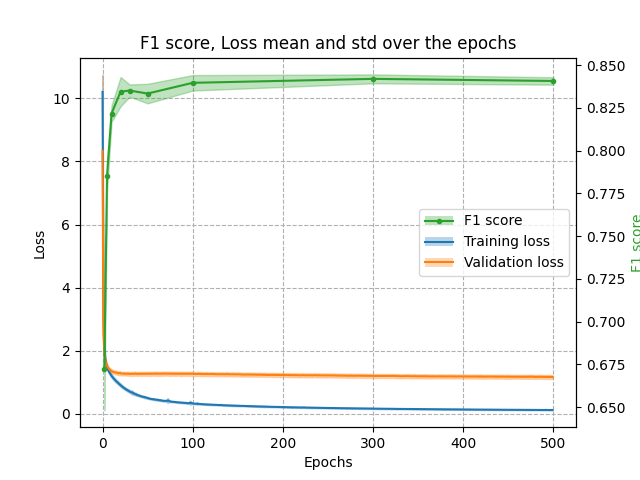
\includegraphics[scale=0.7]{Figures/results/yolov8/yolov8_xs_f1_score_and_loss.png}
    \caption{Visualisation de l'évolution du coût et du score F1 du modèle YOLOv8 xs au fil des époques.}
    \label{fig:yolov8_xs_f1_score_and_loss}
\end{figure}

\newpage

Nous observons une diminution très rapide du coût pour les ensembles d'entraînement et de validation, puis une phase très stable pour le coût des données de validation et beaucoup plus calme pour le coût des données d'entraînement qui continue de diminuer légèrement. Cela nous permet d'assumer que notre modèle est suffisamment entraîné.\\

Concernant les métriques, nous pouvons constater que le rappel et l'AP[.5] diminuent au fil des itérations après un pic, tandis que le score F1 et l'AP[.5,.05,.95] ont tendance à rester relativement stables. La précision quant à elle semble présenter une amélioration de ses résultats suite à une forte diminution de ceux-ci, mais qui reste inférieure au sommet atteint après quelques époques d'entraînement.

Comme nous pouvions nous en douter, les différentes versions affichent lors des premières itérations des différences relatives à leur taille. Néanmoins, comme nous le constatons grâce à la table \ref{tab:mean_f1_scores_yolov8_models}, retraçant les moyennes du score F1 à différentes époques pour toutes les tailles de YOLOv8, ces différences sont relativement faibles : moins de 2\%. La seule métrique où la différence est plus flagrante est l'AP[.5,.05,.95] sur la figure \ref{fig:yolov8_visulization_ap05_095_standard_models}, où nous pouvons voir que la version xs performe moins bien que celles plus grandes.

\begin{table}[!ht]
    \caption{Moyenne des scores F1 des modèles YOLOv8 à 20, 50, 100, et 500 époques}
    \label{tab:mean_f1_scores_yolov8_models}
    \rowcolors{2}{gray!25}{white}
    \centering
    \begin{tabular}{ |c||c|c|c|c|  }
        \hline
        \rowcolor{gray!50}
        Modèle & 20 & 50 & 100 & 500\\
        \hline
        YOLOv8 xs & 0.8345 & 0.8334 & 0.8397 & 0.8408\\
        YOLOv8 s & 0.8441 & 0.8457 & 0.8471 & 0.8471\\
        YOLOv8 m & 0.8520 & 0.8492 & 0.8480 & 0.8418\\
        YOLOv8 l & 0.8517 & 0.8487 & 0.8560 & 0.8443\\
        YOLOv8 xl & 0.8521 & 0.8504 & 0.8514 & 0.8435\\
        \hline
    \end{tabular}
\end{table}

De plus, les résultats des différentes versions démontrent une tendance à converger au fil de l'entraînement. En observant les moyennes des scores F1 à différentes époques de la table \ref{tab:mean_f1_scores_yolov8_models}, nous constatons que les modèles xs, et s ont tendance à continuer de s'améliorer à l'inverse des versions m, l, et xl qui performent moins bien. En observant leur déviation standard à l'aide de la table \ref{tab:std_f1_scores_yolov8_models}, il apparaît que celles des modèles xs, et s diminuent au fil des époques tandis que celle des modèles m, l, et xl augmentent. Nous pouvons supposer que les plus grandes tailles commencent à être surentraînées pendant que les plus petites continuent d'apprendre créant la tendance observée.

\begin{table}[!ht]
    \caption{Ecart-type des scores F1 des modèles YOLOv8 à 20, 50, 100, et 500 époques}
    \label{tab:std_f1_scores_yolov8_models}
    \rowcolors{2}{gray!25}{white}
    \centering
    \begin{tabular}{ |c||c|c|c|c|  }
        \hline
        \rowcolor{gray!50}
        Modèle & 20 & 50 & 100 & 500\\
        \hline
        YOLOv8 xs & 0.0086 & 0.0057 & 0.0045 & 0.0022\\
        YOLOv8 s & 0.0034 & 0.0054 & 0.0057 & 0.0016\\
        YOLOv8 m & 0.0030 & 0.0031 & 0.0035 & 0.0034\\
        YOLOv8 l & 0.0022 & 0.0034 & 0.0045 & 0.0056\\
        YOLOv8 xl & 0.0048 & 0.0048 & 0.0046 & 0.0073\\
        \hline
    \end{tabular}
\end{table}

En s'intéressant aux moyennes des différentes métriques présentées dans la table \ref{tab:max_values_for_each_metric_yolov8_models} toutes époques confondues, nous pouvons étudier plus en détail le comportement de notre modèle face au problème de la détection de jets.

La précision atteint des valeurs autour de 92\% en fonction de la version choisie. Celle-ci est plus que satisfaisante et nous indique que lorsque notre modèle détecte un élément, il s'agit très probablement d'un jet. Le rappel est quant à lui plus faible et atteint 80\%. Cette valeur bien que satisfaisante nous indique que malgré la capacité à détecter une bonne partie des jets présents sur une image, notre modèle en manque un nombre non négligeable. Le score F1 avec des valeurs supérieures à 84\%, nous indique que notre modèle est bien balancé entre les éléments qu'il détecte correctement et la totalité de ceux qu'il doit détecter.

Regardons à présent les AP[.5] et AP[.5,.05,.95]. Avec une AP[.5] au moins supérieure à 81\%, nous voyons que notre modèle est capable de réaliser d'excellentes prédictions pour une \acrshort{iou} de 50\%.

En ce qui concerne l'AP[.5,.05,.95], avec des résultats à partir de 50\%, YOLOv8 propose de bonnes prédictions. Nous pouvons comparer les performances du modèle sur notre problème de détection de jets à celui présenté par Ultralytics sur le jeu de données COCO \cite{ultralytics_detect_nodate} que nous avons reporté sur la table \ref{tab:ultralytics_yolov8_results}. En comparant les deux, nous voyons que YOLOv8 performe mieux sur la détection de jets. Cette différence est flagrante lorsque l'on compare les résultats entre les versions xs. Nous avons 37.3\% contre 50.16\%, ce qui correspond à 12.86\% d'écart. Celui-ci peut s'expliquer par le fait que l'ensemble COCO comprend énormément de classes issues d'images contenant des schémas complexes qui sont mieux appréhendés par les tailles possédant un nombre de filtres par convolution plus élevé. En gardant cela en tête, nous pouvons en déduire que pour la détection de jets, des versions d'une taille plus modeste peuvent suffire a obtenir des bonnes performances.

Nous pouvons appuyer cela par les résultats obtenus en observant la taille des modèles (disponibles dans la table \ref{tab:yolov8_flops_only_legit}), nous observons que pour vingt fois plus de paramètres et trente fois plus d'opérations, nous obtenons au maximum moins de 5\% d'écart entre les versions xs et xl.

\begin{table}[!ht]
    \caption{Valeurs moyennes maximales des métriques des modèles YOLOv8 toutes époques confondues}
    \label{tab:max_values_for_each_metric_yolov8_models}
    \rowcolors{2}{gray!25}{white}
    \centering
    \begin{tabular}{ |c||c|c|c|c|c|  }
        \hline
        \rowcolor{gray!50}
        Modèle & Précision & Rappel & Score F1 & AP[.5] & AP[.5,.05,.95]\\
        \hline
        YOLOv8 xs & 0.9200 & 0.7978 & 0.8420 & 0.8135 & 0.5016\\
        YOLOv8 s & 0.9178 & 0.8071 & 0.8478 & 0.8202 & 0.5299\\
        YOLOv8 m & 0.9148 & 0.8218 & 0.8520 & 0.8272 & 0.5403\\
        YOLOv8 l & 0.9289 & 0.8249 & 0.8560 & 0.8279 & 0.5380\\
        YOLOv8 xl & 0.9281 & 0.8185 & 0.8521 & 0.8333 & 0.5498\\
        \hline
    \end{tabular}
\end{table}

\begin{table}[!ht]
    \caption{Résultats présentés par Ultralytics pour YOLOv8 sur le jeu de données COCO}
    \label{tab:ultralytics_yolov8_results}
    \rowcolors{2}{gray!25}{white}
    \centering
    \begin{tabular}{ |c||c|  }
        \hline
        \rowcolor{gray!50}
        Modèle & AP[.5,.05,.95]\\
        \hline
        YOLOv8 xs & 0.373\\
        YOLOv8 s & 0.449\\
        YOLOv8 m & 0.502\\
        YOLOv8 l & 0.529\\
        YOLOv8 xl & 0.539\\
        \hline
    \end{tabular}
\end{table}

\clearpage

\begin{figure}[!htbp]
    \centering
    \begin{minipage}[t]{.5\textwidth}%\vspace{0pt}
      \centering
      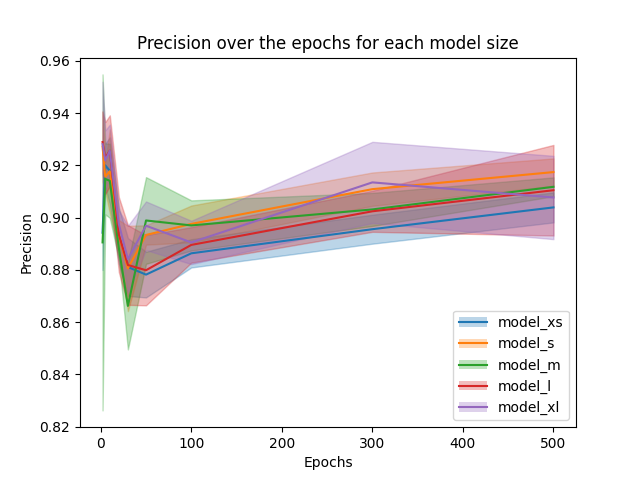
\includegraphics[width=1.1\linewidth]{Figures/results/yolov8/precision_over_epochs_standard_sizes.png}
      \captionof{figure}{Visualisation de la précision pour les différentes tailles de YOLOv8.}
      \label{fig:yolov8_visulization_precision_standard_models}
    \end{minipage}%
    \begin{minipage}[t]{.5\textwidth}%\vspace{5pt}
      \centering
      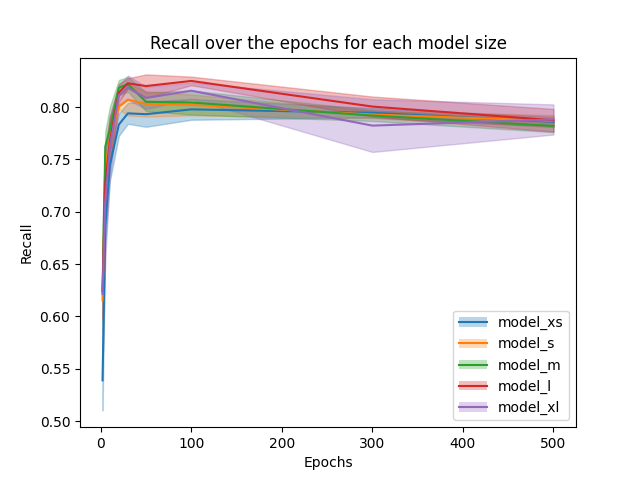
\includegraphics[width=1.1\linewidth ]{Figures/results/yolov8/recall_over_epochs_standard_sizes.png}
      \captionof{figure}{Visualisation du rappel pour les différentes tailles de YOLOv8.}
      \label{fig:yolov8_visulization_recall_standard_models}
    \end{minipage}
\end{figure}

\begin{figure}[!htbp]
    \centering
    \begin{minipage}[t]{.5\textwidth}%\vspace{0pt}
      \centering
      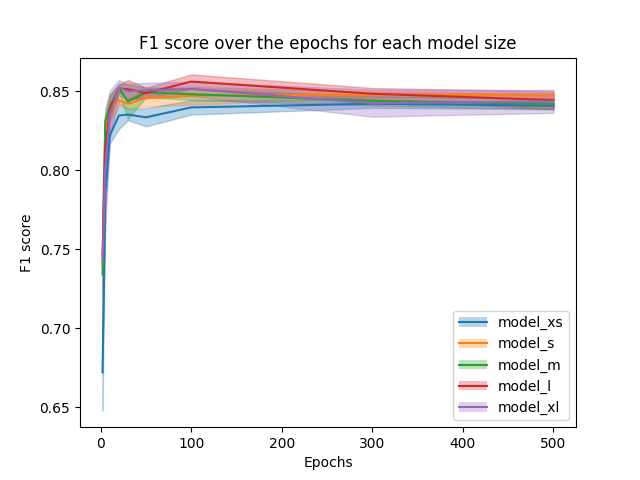
\includegraphics[width=1.1\linewidth]{Figures/results/yolov8/f1_score_over_epochs_standard_sizes.png}
      \captionof{figure}{Visualisation du score F1 pour les différentes tailles de YOLOv8.}
      \label{fig:yolov8_visulization_f1_score_standard_models}
    \end{minipage}%
\end{figure}

\begin{figure}[!htbp]
    \centering
    \begin{minipage}[t]{.5\textwidth}%\vspace{0pt}
      \centering
      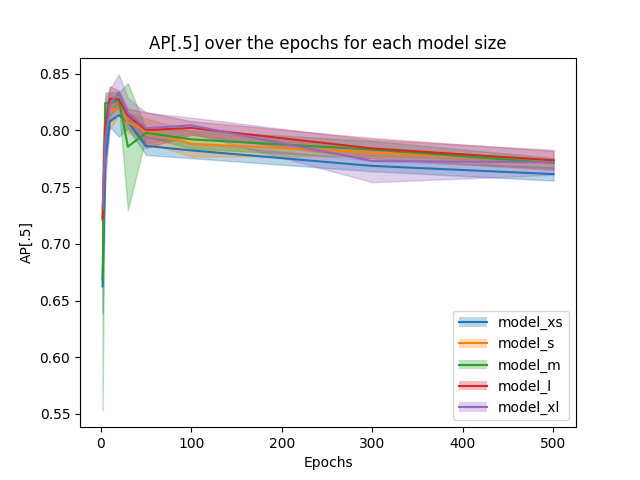
\includegraphics[width=1.1\linewidth]{Figures/results/yolov8/ap05_over_epochs_standard_sizes_standard_models.png}
      \captionof{figure}{Visualisation de l'AP[.5] pour les différentes tailles de YOLOv8.}
      \label{fig:yolov8_visulization_ap05_standard_models}
    \end{minipage}%
    \begin{minipage}[t]{.5\textwidth}%\vspace{5pt}
      \centering
      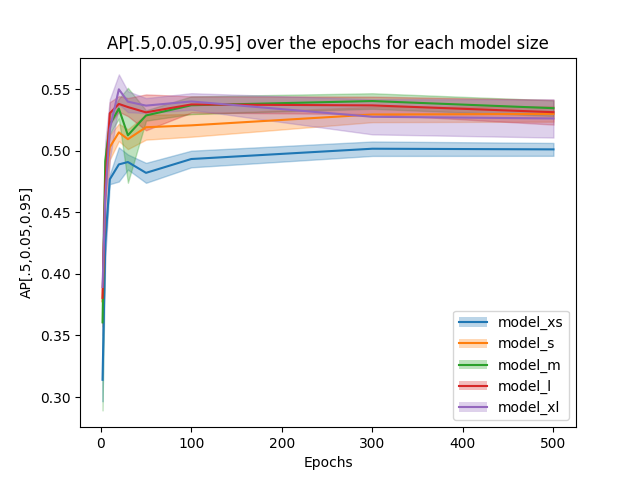
\includegraphics[width=1.1\linewidth ]{Figures/results/yolov8/ap05_095_over_epochs_standard_sizes_standard_models.png}
      \captionof{figure}{Visualisation de l'AP[.5,.05,.95] pour les différentes tailles de YOLOv8.}
      \label{fig:yolov8_visulization_ap05_095_standard_models}
    \end{minipage}
\end{figure}

\clearpage


%--------------------------------------
% Courbes précision x rappel
%--------------------------------------
\subsection{Résultats YOLOv8 : courbe précision-rappel}

Observons à présent la relation entre la précision et le rappel pour une \acrshort{iou} de 50\% et de 95\% respectivement sur les figures \ref{fig:yolov8_visulization_apxr05_standard_models}, et \ref{fig:yolov8_visulization_apxr095_standard_models}. La première affiche une précision relativement stable, voire diminuant très légèrement, jusqu'à un rappel d'environ 80\%, moment à partir duquel la précision chute brutalement jusqu'à 0. Cela nous indique que pour pratiquement une même précision, nous pouvons obtenir un bon rappel jusqu'à un peu moins de 80\%. Bien qu'il ne s'agisse pas d'une courbe parfaite, la relation entre la précision et le rappel est très bonne. Par ailleurs, le même comportement est observé auprès des différentes versions de YOLOv8. En effet, nous pouvons voir que la taille m débute avec une précision plus faible. Cela signifie que lors de l'inférence, le modèle a attribué le score de confiance le plus élevé à des prédictions fausses.

\begin{figure}[hbt!]
    \centering
    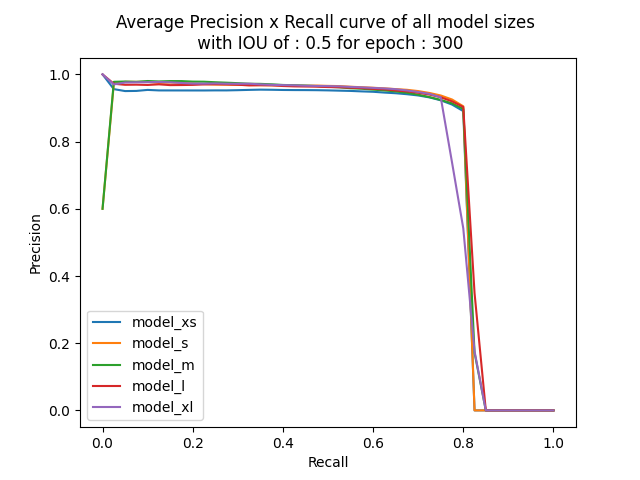
\includegraphics[scale=0.7]{Figures/results/yolov8/apxr_05_300.png}
    \caption{Visualisation de la moyenne des courbes précision x rappel avec un \acrshort{iou} de 0.5 pour les différentes tailles de YOLOv8 après 300 époques.}
    \label{fig:yolov8_visulization_apxr05_standard_models}
\end{figure}

Sur la deuxième figure en revanche, il ne se passe pas la même chose. La précision diminue progressivement dès un très faible rappel, puis à partir d'un seuil, différent en fonction de la taille, la précision tombe rapidement à zéro. De façon globale dès que le rappel augmente légèrement la précision est quant à elle très faible, jusqu'à un rappel de 40\% moment où toutes les précisions sont à 0.

Ce qui est intéressant est de voir que les différentes tailles n'ont pas toutes les mêmes valeurs. Nous remarquons que sur cette visualisation, la courbe du modèle xs est beaucoup plus faible que les autres. Les courbes des tailles s, l, xl ont relativement le même comportement, hormis le début de la courbe xl qui est la seule commençant à 1. La courbe de la taille m obtient quelques meilleurs résultats, mais finit tout de même par converger au même point que les courbes précédentes.

Les résultats sont évidemment moins bons sur la figure \ref{fig:yolov8_visulization_apxr095_standard_models}, car l'\acrshort{iou} est beaucoup plus élevé. Cela implique que pour qu'une détection soit validée, celle-ci doit être détectée avec beaucoup plus de précision sur l'image. Cette contrainte nous permet d'évaluer la capacité des différentes versions à gérer la précision et le rappel avec une \acrshort{iou} de 95\%.

Contrairement à la figure \ref{fig:yolov8_visulization_apxr05_standard_models} où rien ne se démarquait réellement entre les différentes tailles, nous voyons que le modèle xs a plus de mal à obtenir les mêmes résultats que les autres tailles. Cela nous permet donc de comprendre que malgré de bonnes performances dans la métrique AP[.5,.05,.95], le plus petit modèle à beaucoup plus de mal à obtenir de vraies détections avec une \acrshort{iou} d'au moins 95\%. Ainsi, si le critère principal est d'être le plus précis possible pour la zone de détection, YOLOv8 xs sera moins adaptée.

\begin{figure}[hbt!]
    \centering
    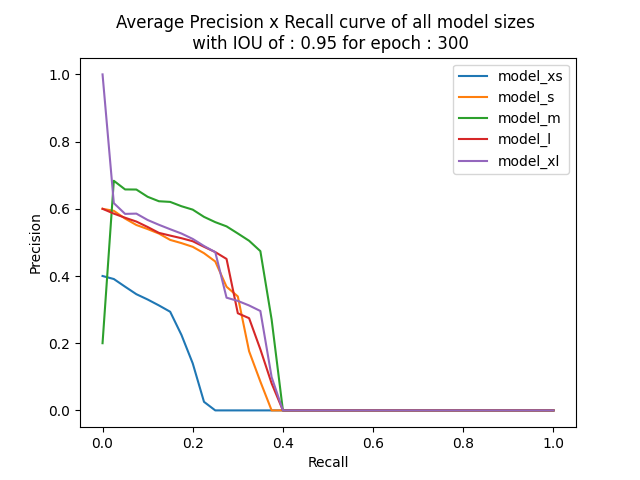
\includegraphics[scale=0.7]{Figures/results/yolov8/apxr_095_300.png}
    \caption{Visualisation de la moyenne des courbes précision x rappel avec un \acrshort{iou} de 0.95 pour les différentes tailles de YOLOv8 après 300 époques.}
    \label{fig:yolov8_visulization_apxr095_standard_models}
\end{figure}

%--------------------------------------
% Nombre de FLOPS / Vitesse
%--------------------------------------

\subsection{Résultats YOLOv8 : FLOPS et vitesse}
\label{subsec:results_yolov8_flops_vitesse}

Analysons les \acrfull{flops} et la vitesse des différentes tailles de YOLOv8 affichée sur la table \ref{tab:yolov8_flops_only_legit}.

En regardant le nombre de paramètres ou les \acrshort{flops}, nous constatons sans surprise qu'à mesure que la taille du modèle augmente, le nombre d'opérations à effectuer augmente également. En comparant les modèles xs et s dont la différence est le nombre de filtres de convolution qui est doublé, ou encore les tailles l et xl dont le nombre de filtres de convolution est 1.5 fois plus élevé. Nous constatons que la relation entre le nombre de filtres de convolution utilisés et le nombre de paramètres ou \acrshort{flops} est quadratique.

En ce qui concerne la vitesse et le nombre d'images par seconde traité par le modèle sur une carte graphique, nous observons que peu importe la taille, le temps est toujours inférieur à 1 ms et compris dans un faible intervalle. En comparant la différence de vitesse entre les tailles xs et s nous voyons que celle-ci est très faible.

Avec plus de 1500 images par secondes pour le modèle le plus grand, YOLOv8 tient ses promesses en termes de vitesse de détection et performances. Dépassant les 2000 \acrshort{fps}, les modèles xs et s se distinguent à nouveau de par leurs capacités impressionnantes pour un nombre de paramètres et d'opérations relativement faible.

\begin{table}[!ht]
    \caption{Nombre de paramètres, FLOPS, vitesse, et images par secondes pour chaque modèle de YOLOv8}
    \label{tab:yolov8_flops_only_legit}
    \rowcolors{2}{gray!25}{white}
    \centering
    \begin{tabular}{ |c||c|c|c|c| }
        \hline
        \rowcolor{gray!50}
        Modèle & Paramètres (M) & FLOPS (M) & Vitesse (ms) RTX 4070 & FPS\\
        \hline
        YOLOv8 xs & 3.225894 & 79.018728 & 0.41 & 2458\\
        YOLOv8 s & 12.856342 & 313.450472 & 0.43 & 2305\\
        YOLOv8 m & 25.665798 & 778.713192 & 0.49 & 2042\\
        YOLOv8 l & 39.401462 & 1512.913384 & 0.55 & 1806\\
        YOLOv8 xl & 61.535974 & 2362.226408 & 0.60 & 1651\\
        \hline
    \end{tabular}
\end{table}

\subsection{Résultats des versions réduites de YOLOv8 xs}

Avec les informations obtenues et déduites précédemment, et dans l'optique d'une implémentation sur \acrshort{fpga}, ou du moins, sa comparaison avec une version synthétisable pour laquelle nous avons besoin de diminuer le nombre de paramètres du modèle, nous allons observer le comportement du modèle YOLOv8 xs lorsque celui-ci est réduit. Nous allons diviser progressivement le nombre de filtres des couches de convolutions par $2$, $4$, $8$, et $16$.

Les résultats sont présentés sur les figures : \ref{fig:yolov8_visulization_precision_reduced_models}, \ref{fig:yolov8_visulization_recall_reduced_models}, \ref{fig:yolov8_visulization_f1_score_reduced_models}, \ref{fig:yolov8_visulization_ap05_reduced_models}, et \ref{fig:yolov8_visulization_ap05_095_reduced_models}, avec les mêmes métriques que pour les versions officielles de YOLOv8.

\begin{figure}[!htbp]
    \centering
    \begin{minipage}[t]{.5\textwidth}%\vspace{0pt}
      \centering
      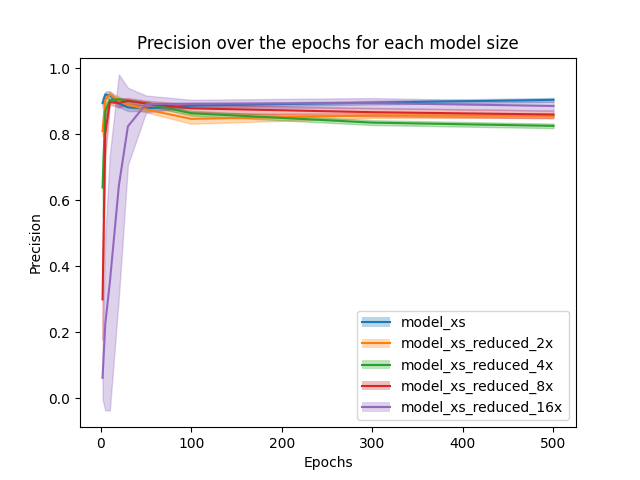
\includegraphics[width=1.1\linewidth]{Figures/results/yolov8/precision_over_epochs_reduced_models.png}
      \captionof{figure}{Visualisation de la précision pour les versions réduites de YOLOv8 xs.}
      \label{fig:yolov8_visulization_precision_reduced_models}
    \end{minipage}%
    \begin{minipage}[t]{.5\textwidth}%\vspace{5pt}
      \centering
      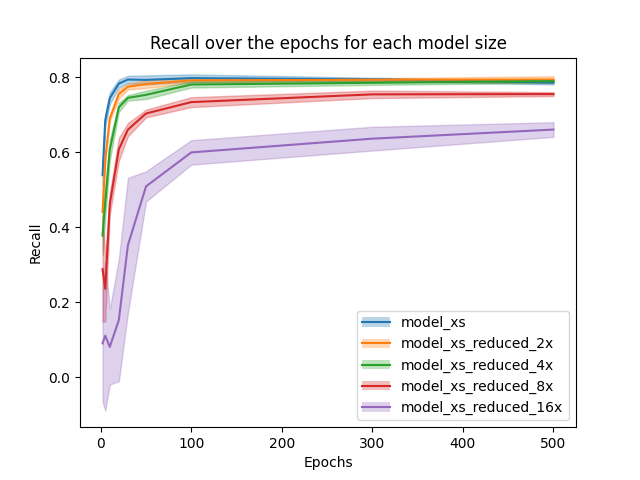
\includegraphics[width=1.1\linewidth ]{Figures/results/yolov8/recall_over_epochs_reduced_models.png}
      \captionof{figure}{Visualisation du rappel pour les versions réduites de YOLOv8 xs.}
      \label{fig:yolov8_visulization_recall_reduced_models}
    \end{minipage}
\end{figure}

\begin{figure}[!htbp]
    \centering
    \begin{minipage}[t]{.5\textwidth}%\vspace{0pt}
      \centering
      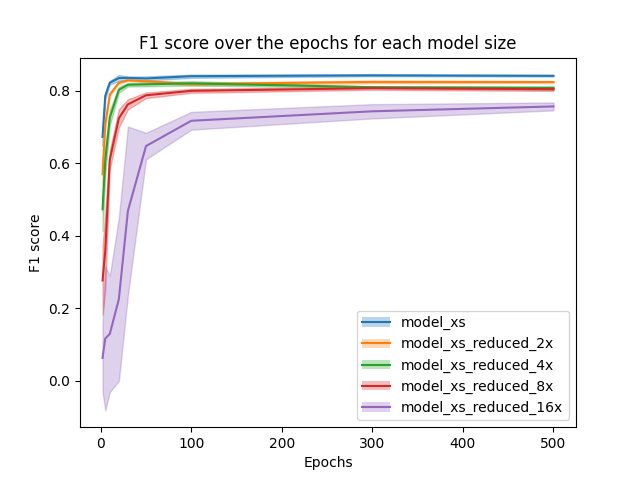
\includegraphics[width=1.1\linewidth]{Figures/results/yolov8/f1_score_over_epochs_reduced_models.png}
      \captionof{figure}{Visualisation du score F1 pour les versions réduites de YOLOv8 xs.}
      \label{fig:yolov8_visulization_f1_score_reduced_models}
    \end{minipage}%
\end{figure}

\begin{figure}[!htbp]
    \centering
    \begin{minipage}[t]{.5\textwidth}%\vspace{0pt}
      \centering
      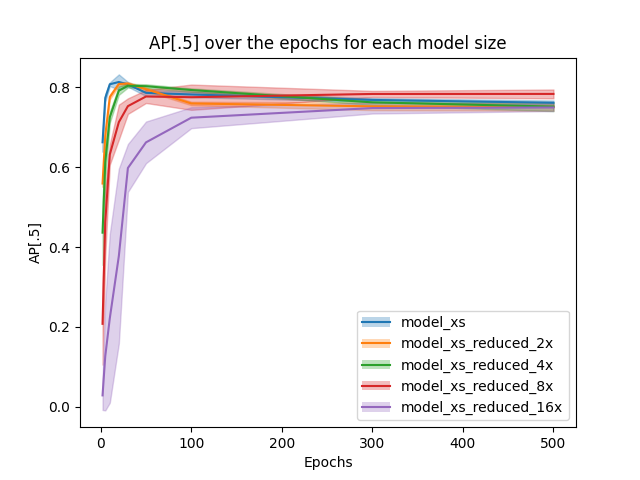
\includegraphics[width=1.1\linewidth]{Figures/results/yolov8/ap05_over_epochs_reduced_models.png}
      \captionof{figure}{Visualisation de l'AP[.5] pour les versions réduites de YOLOv8 xs.}
      \label{fig:yolov8_visulization_ap05_reduced_models}
    \end{minipage}%
    \begin{minipage}[t]{.5\textwidth}%\vspace{5pt}
      \centering
      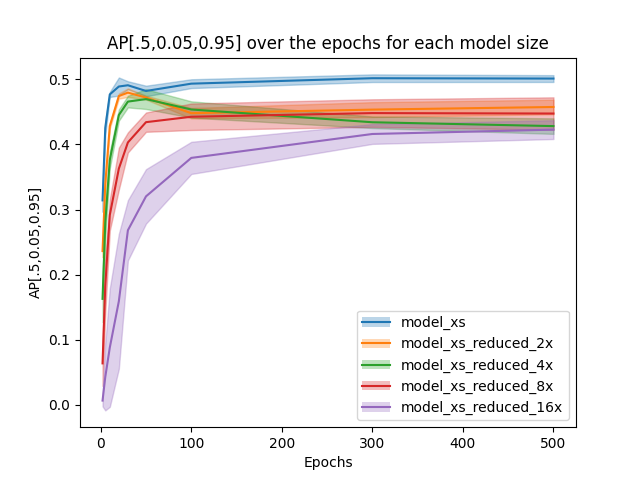
\includegraphics[width=1.1\linewidth ]{Figures/results/yolov8/ap05_095_over_epochs_reduced_models.png}
      \captionof{figure}{Visualisation de l'AP[.5,.05,.95] pour les versions réduites de YOLOv8 xs.}
      \label{fig:yolov8_visulization_ap05_095_reduced_models}
    \end{minipage}
\end{figure}

\break

Lorsque nous regardons les diverses figures, nous constatons que la diminution des filtres impacte plus la qualité des résultats que les différences entre les modèles officiels de YOLOv8. Le rappel \ref{fig:yolov8_visulization_recall_reduced_models}, le score F1 \ref{fig:yolov8_visulization_f1_score_reduced_models}, l'AP[.5] \ref{fig:yolov8_visulization_ap05_reduced_models}, ou encore l'AP[.5,.05,.95] \ref{fig:yolov8_visulization_ap05_095_reduced_models} affichent une nette différence des résultats entre les tailles. Prenons la table \ref{tab:mean_f1_scores_yolov8_reduced_models} affichant les valeurs moyennes du score F1, nous pouvons y voir très clairement que les plus petits modèles ont besoin de plus d'époques d'entraînement pour obtenir de bonnes performances. En effet, en ayant moins de paramètres, les modèles ont plus de mal à capturer les motifs, et nécessitent plus d'entraînement afin de réussir à généraliser ce qu'ils apprennent.

Un élément venant appuyer cela, visible sur la figure \ref{fig:yolov8_visulization_f1_score_reduced_models}, et sur la table \ref{tab:std_f1_scores_yolov8_reduced_models}, concerne l'écart-type du modèle xs réduit 16 fois qui est plus élevé que pour les autres versions. Cela démontre une sensibilité du modèle dans les premières époques qui diminue au fil de l'entraînement, qui peut être dû à l'initialisation des poids, mais aussi aux données.

\begin{table}[!ht]
    \caption{Moyenne des scores F1 des modèles YOLOv8 xs réduits à 20, 50, 100, et 500 époques}
    \label{tab:mean_f1_scores_yolov8_reduced_models}
    \rowcolors{2}{gray!25}{white}
    \centering
    \begin{tabular}{ |c||c|c|c|c|  }
        \hline
        \rowcolor{gray!50}
        Modèle & 20 & 50 & 100 & 500\\
        \hline
        YOLOv8 xs reduced 16x & 0.2250 & 0.6471 & 0.7168 & 0.7564\\
        YOLOv8 xs reduced 8x & 0.7236 & 0.7870 & 0.7994 & 0.8039\\
        YOLOv8 xs reduced 4x & 0.8021 & 0.8172 & 0.8200 & 0.8071\\
        YOLOv8 xs reduced 2x & 0.8215 & 0.8258 & 0.8180  & 0.8236\\
        YOLOv8 xs & 0.8345 & 0.8334 & 0.8397 & 0.8408\\
        \hline
    \end{tabular}
\end{table}

\begin{table}[!ht]
    \caption{Ecart-type des scores F1 des modèles YOLOv8 xs réduits à 20, 50, 100, et 500 époques}
    \label{tab:std_f1_scores_yolov8_reduced_models}
    \rowcolors{2}{gray!25}{white}
    \centering
    \begin{tabular}{ |c||c|c|c|c|  }
        \hline
        \rowcolor{gray!50}
        Modèle & 20 & 50 & 100 & 500\\
        \hline
        YOLOv8 xs reduced 16x & 0.2250 & 0.0364 & 0.0245 & 0.0109\\
        YOLOv8 xs reduced 8x & 0.0253 & 0.0078 & 0.0055 & 0.0049\\
        YOLOv8 xs reduced 4x & 0.0079 & 0.0053 & 0.0061 & 0.0049\\
        YOLOv8 xs reduced 2x & 0.0020 & 0.0026 & 0.0035  & 0.0026\\
        YOLOv8 xs & 0.0107 & 0.0121 & 0.0099 & 0.0049\\
        \hline
    \end{tabular}
\end{table}

\break

Observons les valeurs moyennes maximales obtenues pour chaque métrique par nos modèles réduits. Comme visible sur la figure \ref{fig:yolov8_visulization_precision_reduced_models}, toutes les versions obtiennent des valeurs relativement proches de 90\% avec moins de 3\% de différence. Néanmoins outre cette métrique, les autres possèdent toutes un écart bien plus important. Malgré des performances relativement proches entre la taille xs et sa version divisée par 2 avec au plus 2.21\% d'écart à l'AP[.5,.05,.95], dès que les filtres de convolution sont réduits par un facteur 4 les résultats diminuent fortement.

Nous obtenons ainsi une précision entre 89 - 92\% qui est très satisfaisante. Par ailleurs, cette dernière est relativement proche de celle trouvée pour les tailles officielles de YOLOv8.

Le rappel, avec une majorité des versions autour de 75 - 79\%, est satisfaisant. Il est assez proche des modèles officiels, bien que légèrement moins performants. Pour la plus petite version, nous observons un rappel de 66\% qui est assez pauvre.

Le score F1, nous indique que la valeur la plus faible est de 75\%. Bien que celle-ci soit acceptable, nous savons grâce au score de précision et de rappel que la version la plus petite peine à détecter l'ensemble des jets sur une image. En ce qui concerne les autres, elles ont toutes un score supérieur à 80\% ce qui en font des modèles relativement bien équilibrés.

L'AP[.5] est d'au moins 74\%, nous voyons que nos modèles sont capables d'effectuer de bonnes détections. En regardant l'AP[.5,.05,.95] dont la valeur minimale est de 42.27\%, nous constatons que nos modèles ont plus de mal à réaliser des détections lorsque l'\acrshort{iou} augmente. Néanmoins, les résultats restent toujours supérieurs à ceux obtenus par YOLOv8 xs voire s sur le jeu de données COCO.\\

Comme nous pouvions nous en douter, en diminuant la taille des filtres, les performances ont également diminué. Cependant, les versions divisées par 2, 4, voire 8, présentent seulement quelques pour cent de différences par rapport aux valeurs moyennes des versions s, m, l, et xl pour la majorité des métriques. Les limitations de ces versions réduites sont en revanche notables dans les performances de l'AP[.5,.05,.95] pour lequel la différence est plus élevée.

Néanmoins, malgré la limitation des modèles réduits à détecter des éléments avec un taux d'intersection sur union très élevé, la forte réduction des paramètres et d'opérations qu'ils présentent par rapport à la faible diminution des performances en font des réseaux intéressants dans un contexte de ressources limitées.

\begin{table}[!ht]
    \caption{Valeurs moyennes maximales des métriques des modèles YOLOv8 réduits toutes époques confondues}
    \label{tab:max_values_for_each_metric_yolov8_reduced_models}
    \rowcolors{2}{gray!25}{white}
    \centering
    \begin{tabular}{ |c||c|c|c|c|c|  }
        \hline
        \rowcolor{gray!50}
        Modèle & Précision & Rappel & Score F1 & AP[.5] & AP[.5,.05,.95]\\
        \hline
        \begin{tabular}{@{}c@{}}YOLOv8 xs \\ reduced 16x\end{tabular} & 0.8943 & 0.6606 & 0.7564 & 0.7497 & 0.4227\\
        \begin{tabular}{@{}c@{}}YOLOv8 xs \\ reduced 8x\end{tabular} & 0.9008 & 0.7552 & 0.8065 & 0.7836 & 0.4481\\
        \begin{tabular}{@{}c@{}}YOLOv8 xs \\ reduced 4x\end{tabular} & 0.9055 & 0.7899 & 0.8200 & 0.8042 & 0.4695\\
        \begin{tabular}{@{}c@{}}YOLOv8 xs \\ reduced 2x\end{tabular} & 0.9200 & 0.7939 & 0.8258 & 0.8093 & 0.4795\\
        YOLOv8 xs & 0.9200 & 0.7978 & 0.8420 & 0.8135 & 0.5016\\
        \hline
    \end{tabular}
\end{table}

\clearpage

%--------------------------------------
% Precision x Recall curve
%--------------------------------------

\subsection{Résultats YOLOv8 réduit : courbe précision-rappel}

Prenons les courbes entre la précision et le rappel pour les \acrshort{iou} de 50\% et de 95\% sur les figures \ref{fig:yolov8_visulization_apxr05_reduced_models}, et \ref{fig:yolov8_visulization_apxr095_reduced_models}.

Sur la première, nous pouvons observer que les différentes versions réduites ont un comportement similaire. Nous voyons qu'elles ne démarrent pas à un, car leurs détections avec le score de confiance le plus élevé correspondent à des faux négatifs, en moyenne cela arrive plus ou moins fréquemment en fonction de la taille. La version la plus réduite diminue vers 0 légèrement plus vite que les autres modèles. Néanmoins, le comportement et les valeurs sont plutôt similaires à la courbe \ref{fig:yolov8_visulization_apxr05_standard_models} avec les modèles officiels de YOLOv8, et donc la relation entre la précision et le rappel pour une \acrshort{iou} de 50\% est très bonne.

\begin{figure}[hbt!]
    \centering
    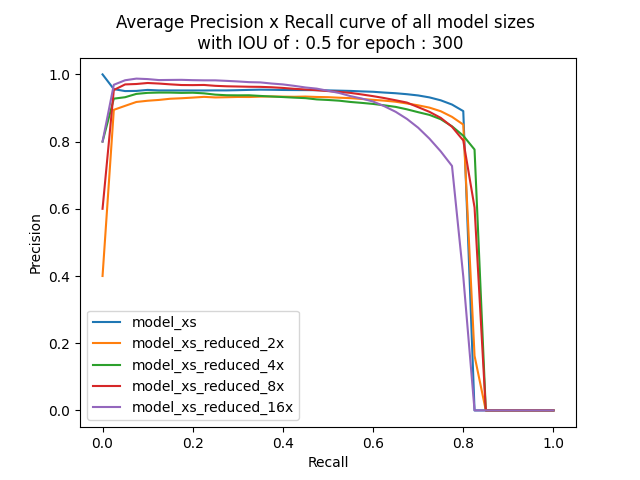
\includegraphics[scale=0.7]{Figures/results/yolov8/apxr_05_300_reduced_models.png}
    \caption{Visualisation de la moyenne des courbes précision x rappel avec un \acrshort{iou} de 0.5 pour les différentes tailles de YOLOv8 réduites après 300 époques.}
    \label{fig:yolov8_visulization_apxr05_reduced_models}
\end{figure}

Sur la deuxième figure \ref{fig:yolov8_visulization_apxr095_reduced_models}, nous voyons que les tailles réduites performent vraiment moins bien que le modèle s qui performe lui-même moins bien que les autres versions officielles. Dans le cadre d'une \acrshort{iou} de 95\%, la relation précision rappel est très pauvre, c'est-à-dire que les modèles de plus petite taille réalisent plus de fausses détections lorsqu'il faut être plus précis sur les zones à détecter.

\begin{figure}[hbt!]
    \centering
    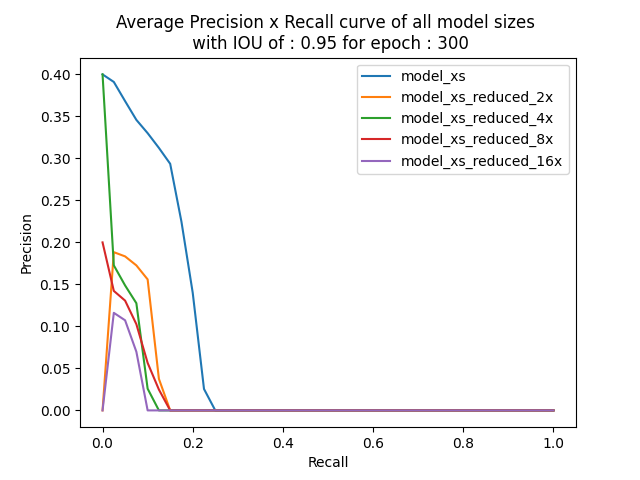
\includegraphics[scale=0.7]{Figures/results/yolov8/apxr_095_300_reduced_models.png}
    \caption{Visualisation de la moyenne des courbes précision x rappel avec un \acrshort{iou} de 0.5 pour les différentes tailles de YOLOv8 réduites après 300 époques.}
    \label{fig:yolov8_visulization_apxr095_reduced_models}
\end{figure}

\break

%--------------------------------------
% Nombre de FLOPS / Vitesse
%--------------------------------------

\subsection{Résultats YOLOv8 réduit : FLOPS et vitesse}

Intéressons nous au nombre de paramètres, d'opérations, ou encore la vitesse de ces versions réduites. Contrairement aux versions de YOLOv8 officielles, nous constatons que la différence de vitesse entre les différentes tailles qui varie entre 0.39 et 0.41 ms n'est pas très importante (voire négligeable étant donné l'échelle), malgré une diminution importante des opérations. Cela peut être dû à diverses raisons, par exemple : des contraintes matérielles, ou encore une parallélisation des opérations très efficaces.
Ces mesures sont à titre indicatives et sont là uniquement pour permettre d'avoir une meilleure idée de ce que le nombre de \acrshort{flops} représente.

En s'intéressant à ces derniers, nous constatons que lorsque nous divisons le nombre de filtres de convolution par 2, nous conservons le rapport quadratique avec le nombre d'opérations. Or, lorsque nous atteignons un nombre de filtres relativement faible, le nombre d'opérations arrête de suivre cette tendance. En effet, le modèle étant composé d'autres couches que des convolutions utilisant différentes tailles de filtres, nous atteignons un nombre de \acrshort{flops}, où leur présence n'est plus négligeable.

\begin{table}[!ht]
    \caption{Nombre de paramètres, FLOPS, vitesse, et images par secondes pour chaque modèle de YOLOv8 réduit}
    \label{tab:yolov8_reduced_flops_only_legit}
    \rowcolors{2}{gray!25}{white}
    \centering
    \begin{tabular}{ |c||c|c|c|c| }
        \hline
        \rowcolor{gray!50}
        Modèle & Paramètres (M) & FLOPS (M) & Vitesse (ms) RTX 4070 & FPS\\
        \hline
        \begin{tabular}{@{}c@{}}YOLOv8 xs \\ reduced 16x\end{tabular} & 0.025779 & 0.961128 & 0.39 & 2566\\
        \begin{tabular}{@{}c@{}}YOLOv8 xs \\ reduced 8x\end{tabular} & 0.0679 & 2.048744 & 0.40 & 2466\\
        \begin{tabular}{@{}c@{}}YOLOv8 xs \\ reduced 4x\end{tabular} & 0.225522 & 5.988072 & 0.39 & 2579\\
        \begin{tabular}{@{}c@{}}YOLOv8 xs \\ reduced 2x\end{tabular} & 0.834286 & 20.923112 & 0.41 & 2456\\
        YOLOv8 xs & 3.225894 & 79.018728 & 0.41 & 2458\\
        \hline
    \end{tabular}
\end{table}

\clearpage

\section{Résultats Resnet18 + Tête}

\subsection{Résultats Resnet18 + Tête pour un nombre différent de blocs de détection}

Analysons à présent les résultats obtenus avec notre implémentation de ResNet18 à laquelle nous avons ajouté une tête afin de réaliser des détections. 

Commençons par regarder l'évolution de la fonction de coût sur l'ensemble d'entraînement et de validation au fil de l'entraînement sur la figure \ref{fig:resnet18+head_loss}. Sur celle-ci, nous voyons que les deux coûts sont très proches l'un de l'autre et indiscernables sur l'image. Par ailleurs, le coût diminue plutôt rapidement avant d'atteindre une stabilité autour des cinquante premières époques. En regardant l'évolution du score F1 en parallèle, nous constatons que celui-ci atteint une valeur très élevée à la cinquantième époque et continue d'augmenter légèrement. Au bout de $500$ époques, nous observons que notre modèle n'a pas eu de grande modification de ses fonctions coûts depuis plus de $400$ époques et que son écart type est également stable. Par ailleurs, à la fin de l'entraînement, il apparaît que le score F1 évolue peu.

\begin{figure}[hbt!]
    \centering
    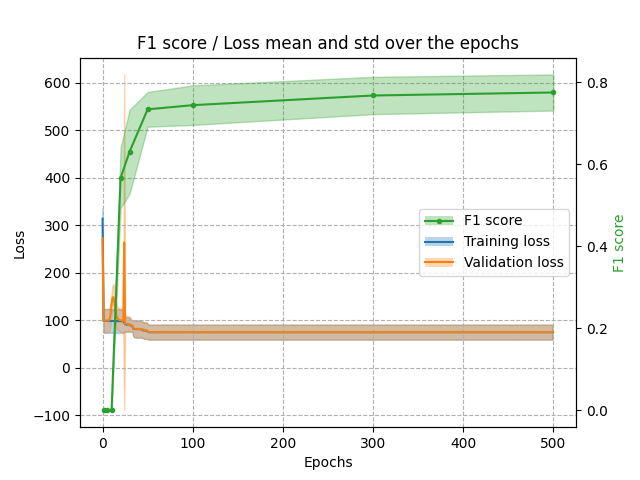
\includegraphics[scale=0.7]{Figures/results/resnet18+head/r18_loss.png}
    \caption{Visualisation de l'évolution du coût et du score F1 du modèle ResNet18+Tête avec 64 D.B. au fil des époques.}
    \label{fig:resnet18+head_loss}
\end{figure}

Les figures \ref{fig:resnet18+head_precision_4_nb_db}, \ref{fig:resnet18+head_recall_4_nb_db}, \ref{fig:resnet18+head_f1_score_4_nb_db}, \ref{fig:resnet18+head_ap05_4_nb_db}, et \ref{fig:resnet18+head_ap05_095_4_nb_db} représentent les moyennes des valeurs obtenues pour les différentes métriques au fil de l'entraînement. Évaluons l'impact du nombre de blocs de détections sur les performances du modèle.

\begin{figure}[!htbp]
    \centering
    \begin{minipage}[t]{.5\textwidth}%\vspace{0pt}
      \centering
      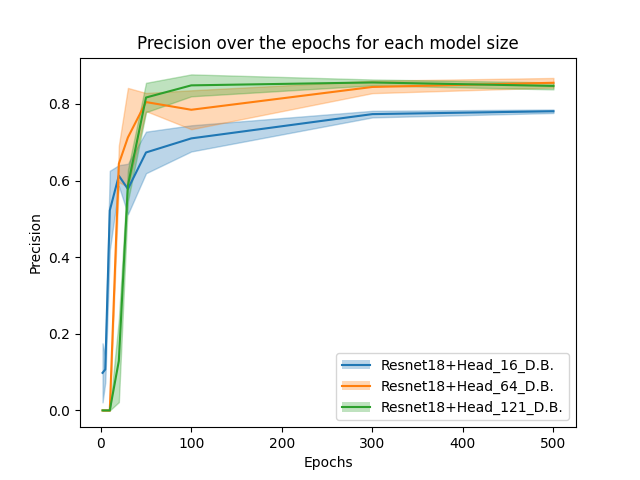
\includegraphics[width=1.1\linewidth]{Figures/results/resnet18+head/resnet18+head_precision_4_nb_db.png}
      \captionof{figure}{Visualisation de la précision de ResNet18+Tête pour un nombre différent de blocs de détection (D.B.).}
      \label{fig:resnet18+head_precision_4_nb_db}
    \end{minipage}%
    \begin{minipage}[t]{.5\textwidth}%\vspace{5pt}
      \centering
      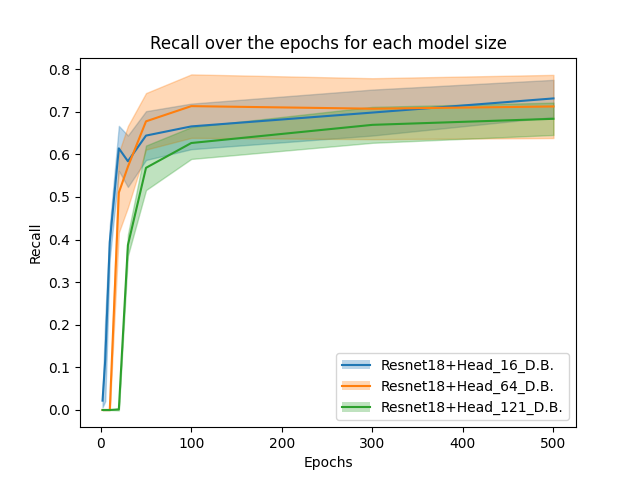
\includegraphics[width=1.1\linewidth ]{Figures/results/resnet18+head/resnet18+head_recall_4_nb_db.png}
      \captionof{figure}{Visualisation du rappel de ResNet18+Tête pour un nombre différent de blocs de détection (D.B.).}
      \label{fig:resnet18+head_recall_4_nb_db}
    \end{minipage}
\end{figure}

\begin{figure}[!htbp]
    \centering
    \begin{minipage}[t]{.5\textwidth}%\vspace{0pt}
      \centering
      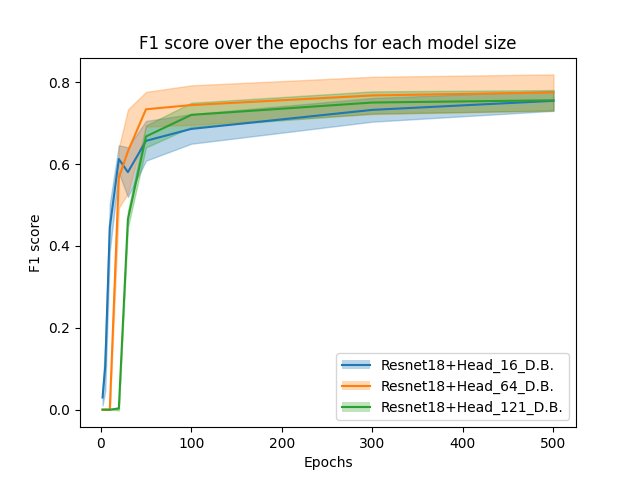
\includegraphics[width=1.1\linewidth]{Figures/results/resnet18+head/resnet18+head_f1_score_4_nb_db.png}
      \captionof{figure}{Visualisation du score F1 de ResNet18+Tête pour un nombre différent de blocs de détection (D.B.).}
      \label{fig:resnet18+head_f1_score_4_nb_db}
    \end{minipage}%
\end{figure}

\begin{figure}[!htbp]
    \centering
    \begin{minipage}[t]{.5\textwidth}%\vspace{0pt}
      \centering
      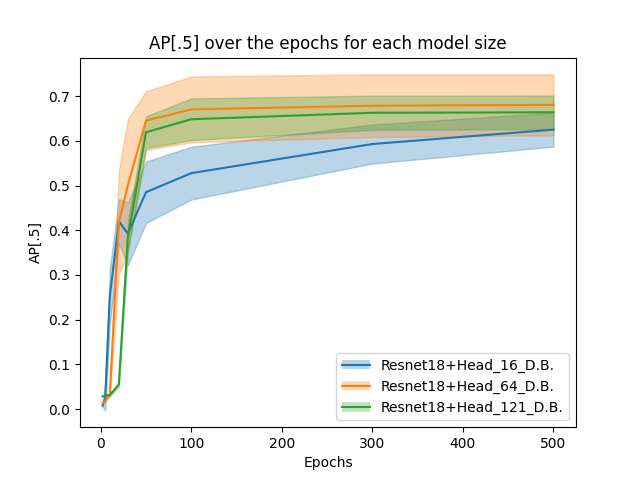
\includegraphics[width=1.1\linewidth]{Figures/results/resnet18+head/resnet18+head_ap05_4_nb_db.png}
      \captionof{figure}{Visualisation de l'AP[.5] de ResNet18+Tête pour un nombre différent de blocs de détection (D.B.).}
      \label{fig:resnet18+head_ap05_4_nb_db}
    \end{minipage}%
    \begin{minipage}[t]{.5\textwidth}%\vspace{5pt}
      \centering
      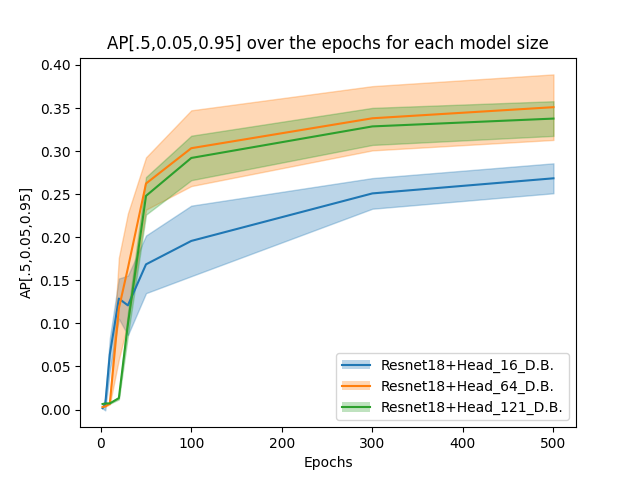
\includegraphics[width=1.1\linewidth ]{Figures/results/resnet18+head/resnet18+head_ap05_95_4_nb_db.png}
      \captionof{figure}{Visualisation de l'AP[.5,.05,.95] de ResNet18+Tête pour un nombre différent de blocs de détection (D.B.).}
      \label{fig:resnet18+head_ap05_095_4_nb_db}
    \end{minipage}
\end{figure}

\break

Un point récurrent à toutes les figures est que la version comportant 16 blocs de détections obtient de meilleurs résultats dans les premières époques d'entraînement comparé aux versions à 64 et 121 blocs, qui est également vérifiable sur les tables \ref{tab:resnet18+head_16n_metrics_avg}, \ref{tab:resnet18+head_64n_metrics_avg}, et \ref{tab:resnet18+head_121n_metrics_avg}. Cette tendance s'inverse assez rapidement, autour des trente à cinquante premières époques. Cela peut s'expliquer par le fait que chaque bloc de détection se voit attribuer beaucoup plus de jets, car le modèle travaille avec quatre à huit fois moins de blocs. Il apprend donc plus rapidement à effectuer des détections.

Cependant, chaque bloc couvrant une plus grande surface que la taille d'un jet et ne pouvant réaliser qu'une détection, ceux-ci ont plus de mal à performer lorsqu'ils doivent détecter précisément le centre d'un jet comme il est possible de l'observer sur la métrique AP@[.5:.95] avec quasiment 9\% d'écart avec la version à 64 blocs, ou encore avec la précision avec plus de 7\% de différence. En revanche, le meilleur score de rappel est obtenu par cette version plus petite, très probablement, car chaque neurone couvrant un nombre de pixels sur l'image plus élevé, il y a moins de problèmes de détection d'un même jet par deux neurones différents.\\

Plusieurs époques plus tard, les modèles comportant 64 et 121 blocs de détection obtiennent à leur tour de meilleurs résultats que la version à 16 blocs. Néanmoins, ils affichent de meilleurs résultats pour les 64 blocs. Augmenter simplement le nombre de blocs de détections ne permet donc pas d'obtenir de meilleurs résultats. Il faut donc trouver la valeur optimisant ceux-ci. Le modèle de 64 blocs va travailler sur des portions de $8 \times 8$ pixels correspondant environ au diamètre d'un jet, contrairement au modèle de 121 blocs dont la surface de travail est de $4 \times 4$. Avec une granularité trop fine, les blocs pourraient voir moins de jets lors de l'entraînement ce qui pourrait expliquer cette différence.\\

En ce qui concerne les performances, il est intéressant de voir que la version avec 64 blocs de détections est celle obtenant globalement les meilleurs résultats. Avec une précision moyenne de 85.51\%, très proche de celle avec 121 blocs, nous obtenons une précision très bonne. 

Le meilleur rappel moyen étant de 71.29, nous avons là également un rappel acceptable. Le score F1 moyen étant de 77.5\%, nous voyons que notre modèle est capable dans l'ensemble d'effectuer de bonnes détections.

Par rapport à l'AP, nous constatons que lorsque l'\acrshort{iou} est de 50\%, nous atteignons une moyenne de 68.04\%. Cette valeur nous indique que bien que le modèle arrive à effectuer des détections correctes, il reste encore de la marge pour des améliorations. Lorsque nous nous attardons sur la valeur de l'AP de 0.5 à 0.95 avec un pas de 0.05, nous voyons que nous obtenons 35.10\% ce qui est un résultat modéré. Néanmoins, cette métrique incorporant des seuils d'intersections sur union plus stricts, il n'est pas étonnant de voir qu'elle est inférieure à l'AP[.5].

\begin{table}[!ht]
    \caption{Valeurs moyenne des métriques du modèle Resnet18 + Tête avec 16 blocs de détection au fil de l'entraînement}
    \label{tab:resnet18+head_16n_metrics_avg}
    \rowcolors{2}{gray!25}{white}
    \centering
    \begin{tabular}{ |c||c|c|c|c|c|  }
        \hline
        \rowcolor{gray!50}
        Epoque & Précision & Rappel & Score F1 & AP[.5] & AP[.5,.05,.95]\\
        \hline
        2 & 0.0980 & 0.0220 & 0.0298 & 0.0079 & 0.0017\\
        5 & 0.1068 & 0.1183 & 0.1056 & 0.0264 & 0.0062\\
        10 & 0.5220 & 0.3943  & 0.4454 & 0.2512 & 0.0638\\
        20 & 0.6126 & 0.6139 & 0.6122 & 0.4201 & 0.1288\\
        30 & 0.5779 & 0.5837 & 0.5803 & 0.3923 & 0.1209\\
        50 & 0.6732 & 0.6438 & 0.6568 & 0.4851 & 0.1686\\
        100 & 0.7100 & 0.6654 & 0.6859 & 0.5277 & 0.1957\\
        300 & 0.7734 & 0.6978 & 0.7324 & 0.5928 & 0.2509\\
        500 & 0.7809 & 0.7310 & 0.7544 & 0.6250 & 0.2684\\
        \hline
    \end{tabular}
\end{table}

\begin{table}[!ht]
    \caption{Valeurs moyenne des métriques du modèle Resnet18 + Tête avec 64 blocs de détection au fil de l'entraînement}
    \label{tab:resnet18+head_64n_metrics_avg}
    \rowcolors{2}{gray!25}{white}
    \centering
    \begin{tabular}{ |c||c|c|c|c|c|  }
        \hline
        \rowcolor{gray!50}
        Epoque & Précision & Rappel & Score F1 & AP[.5] & AP[.5,.05,.95]\\
        \hline
        2 & 0.0000 & 0.0000 & 0.0000 & 0.0139 & 0.0030\\
        5 & 0.0000 & 0.0000 & 0.0000 & 0.0181 & 0.0038\\
        10 & 0.0000 & 0.0000 & 0.0000 & 0.0318 & 0.0068\\
        20 & 0.6437 & 0.5101 & 0.5666 & 0.4173 & 0.1172\\
        30 & 0.7124 & 0.5707 & 0.6308 & 0.5007 & 0.1642\\
        50 & 0.8048 & 0.6773 & 0.7339 & 0.6451 & 0.2624\\
        100 & 0.7847 & 0.7129 & 0.7441 & 0.6703 & 0.3034\\
        300 & 0.8442 & 0.7069 & 0.7676 & 0.6784 & 0.3381\\
        500 & 0.8551 & 0.7122 & 0.7750 & 0.6804 & 0.3510\\
        \hline
    \end{tabular}
\end{table}

\begin{table}[!ht]
    \caption{Valeurs moyenne des métriques du modèle Resnet18 + Tête avec 121 blocs de détection au fil de l'entraînement}
    \label{tab:resnet18+head_121n_metrics_avg}
    \rowcolors{2}{gray!25}{white}
    \centering
    \begin{tabular}{ |c||c|c|c|c|c|  }
        \hline
        \rowcolor{gray!50}
        Epoque & Précision & Rappel & Score F1 & AP[.5] & AP[.5,.05,.95]\\
        \hline
        2 & 0.0000 & 0.0000 & 0.0000 & 0.0286 & 0.0065\\
        5 & 0.0000 & 0.0000 & 0.0000 & 0.0309 & 0.0071\\
        10 & 0.0000 & 0.0000 & 0.0000 & 0.0312 & 0.0072\\
        20 & 0.1294 & 0.0013 & 0.0026 & 0.0554 & 0.0132\\
        30 & 0.5868 & 0.3869 & 0.4652 & 0.3853 & 0.0992\\
        50 & 0.8167 & 0.5682 & 0.6674 & 0.6191 & 0.2480\\
        100 & 0.8484 & 0.6264 & 0.7201 & 0.6482 & 0.2920\\
        300 & 0.8560 & 0.6690 & 0.7503 & 0.6627 & 0.3286\\
        500 & 0.8469 & 0.6832 & 0.7558 & 0.6637 & 0.3377\\
        \hline
    \end{tabular}
\end{table}

\break

Regardons à présent la courbe de la précision et du rappel pour un \acrshort{iou} de 50\% sur la figure \ref{fig:resnet18+head_apxr_05_500_4_nb_db}. Comme nous pouvions nous en douter d'après les résultats obtenus, celle-ci est loin d'être parfaite. Néanmoins, elle démontre tout de même une relation entre la précision et le rappel relativement bonne. Les versions à 64 et 121 blocs de détections s'en tirent globalement mieux, bien que le modèle à 16 blocs les rejoint lorsque le rappel augmente.

Sur la figure \ref{fig:resnet18+head_apxr_095_500_4_nb_db} en revanche, bien qu'il y ait un léger pic, les valeurs sont quasiment toujours nulles. Cela nous indique que notre modèle n'est pas capable de réaliser des détections lorsque le seuil d'intersection sur union est trop élevé.

\begin{figure}[!htbp]
    \centering
    \begin{minipage}[t]{.5\textwidth}%\vspace{0pt}
      \centering
      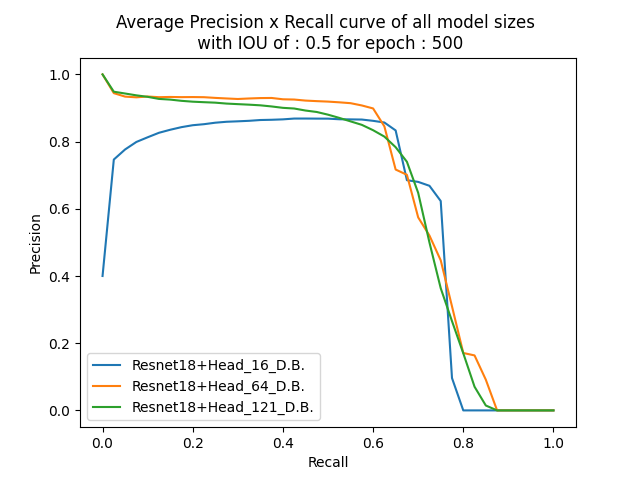
\includegraphics[width=1.1\linewidth]{Figures/results/resnet18+head/resnet18+head_apxr_05_500.png}
      \captionof{figure}{Visualisation de la moyenne des courbes précision x rappel avec un IoU de 0.5 pour ResNet18+Tête avec un nombre différent de blocs de détection (D.B.) après 500 époques.}
      \label{fig:resnet18+head_apxr_05_500_4_nb_db}
    \end{minipage}%
    \begin{minipage}[t]{.5\textwidth}%\vspace{5pt}
      \centering
      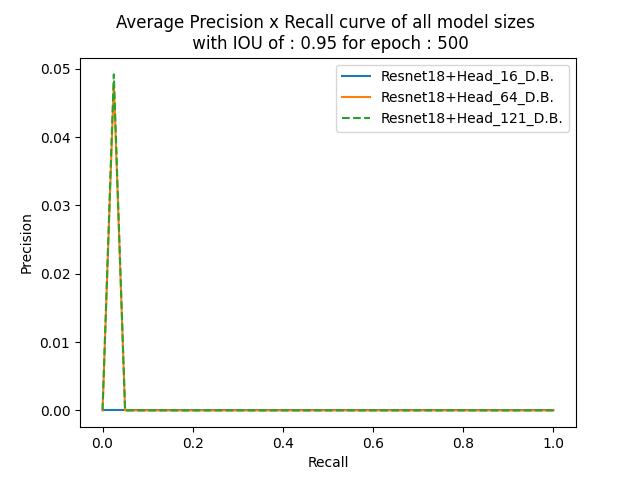
\includegraphics[width=1.1\linewidth ]{Figures/results/resnet18+head/resnet18+head_apxr_095_500.png}
      \captionof{figure}{Visualisation de la moyenne des courbes précision x rappel avec un IoU de 0.95 pour ResNet18+Tête avec un nombre différent de blocs de détection (D.B.) après 500 époques.}
      \label{fig:resnet18+head_apxr_095_500_4_nb_db}
    \end{minipage}
\end{figure}

\break

Finalement, observons le nombre de paramètres, d'opérations et la vitesse des différentes tailles de blocs affichés sur la table \ref{tab:resnet18+head_params_flops_vitesse_fps_4_nb_db}. Sans surprises, le nombre de blocs influe peu sur le nombre de paramètres et d'opérations du modèle.

En revanche, la vitesse d'inférence et par conséquent le nombre d'images par secondes entre la version avec 16 blocs de détection et les versions de 64 et 121 possèdent un très grand écart. A priori, étant donné que les paramètres et le nombre d'opérations sont relativement proches, il serait logique de penser que la différence ne devrait pas être très élevée. Si nous analysons le nombre d'opérations qui sont réalisées, reporté sur la table \ref{tab:resnet18+head_params_node_4_nb_db}, nous constatons que l'opération de produit matriciel (MatMul) est celle qui évolue le plus. Cette dernière uniquement présente dans les couches Dense de notre modèle explique pourquoi elle est liée au nombre de blocs utilisés. Nous pouvons donc raisonnablement supposer que le nombre de produits matriciel à effectuer à une forte incidence sur la vitesse de calcul.

Cependant, avec plus de 3900 images par seconde, et des temps inférieurs à 0.26 ms, nous voyons que les vitesses atteintes restent très élevées dans les trois cas.

\begin{table}[!ht]
    \caption{Nombre de paramètres, FLOPs, vitesse, FPS pour ResNet18+Tête avec 16, 64, et 121 blocs de détection (D.B.)}
    \label{tab:resnet18+head_params_flops_vitesse_fps_4_nb_db}
    \rowcolors{2}{gray!25}{white}
    \centering
    \begin{tabular}{ |c||c|c|c|c| }
        \hline
        \rowcolor{gray!50}
        Modèle & Paramètres (M) & MFLOPs & \begin{tabular}{@{}c@{}}Vitesse (ms) \\ RTX 4070 \end{tabular} & FPS\\
        \hline
        ResNet18+Tête 16 D.B. & 11.215536 & 287.382512 & 0.1150 & 8695\\
        ResNet18+Tête 64 D.B. & 11.289408 & 287.530112 & 0.2142 & 4668\\
        ResNet18+Tête 121 D.B. & 11.377131 & 287.705387 & 0.2508 & 3986\\
        \hline
    \end{tabular}
\end{table}

\begin{table}[!ht]
    \caption{Nombre de paramètres de chaque noeud pour ResNet18+Tête avec 16, 64, et 121 blocs de détection (D.B.)}
    \label{tab:resnet18+head_params_node_4_nb_db}
    \rowcolors{2}{gray!25}{white}
    \centering
    \begin{tabular}{ |c||c|c|c| }
        \hline
        \rowcolor{gray!50}
        Noeud & \begin{tabular}{@{}c@{}}Nb ops R18+Tête \\ 16 D.B. \end{tabular} & \begin{tabular}{@{}c@{}}Nb ops R18+Tête \\ 64 D.B. \end{tabular} & \begin{tabular}{@{}c@{}}Nb ops R18+Tête \\ 121 D.B. \end{tabular}\\
        \hline
        Conv2D & 286.95m & 286.95m & 286.95m\\
        MatMul & 49.15k & 196.61k & 371.71k\\
        BiasAdd & 194.86k & 195.01k & 195.18k\\
        MaxPool & 129.60k & 129.60k & 129.60k\\
        AddV2 & 57.47k & 57.47k & 57.47k\\
        Mean & 2.05k & 2.05k & 2.05k\\
        \hline
    \end{tabular}
\end{table}

\clearpage

\subsection{Résultats Resnet18 + Tête : versions réduites avec 64 blocs de détection}

En réduisant le nombre de filtres de convolution de notre modèle possédant 64 blocs de détection par : 2, 4, 8, 16, et 32 en vue de le synthétiser avec \acrshort{hls4ml}, nous constatons sur les figures \ref{fig:resnet18+head_precision_reduced}, \ref{fig:resnet18+head_recall_reduced}, \ref{fig:resnet18+head_f1_score_reduced}, \ref{fig:resnet18+head_ap05_reduced}, et \ref{fig:resnet18+head_ap05_095_reduced} une nette diminution des performances. Ainsi, si les versions réduites par un facteur 2, et 4 possèdent encore des résultats peu éloignés du modèle de base, les autres possèdent une différence plus marquée. Cela se comprend étant donné la diminution du nombre de paramètres, visible sur la table \ref{tab:resnet18+head_params_flops_vitesse_fps_reduced}, les modèles ont de plus en plus de mal à faire ressortir des images les schémas et les caractéristiques nécessaires à la détection des jets.\\

\begin{figure}[!htbp]
    \centering
    \begin{minipage}[t]{.5\textwidth}%\vspace{0pt}
      \centering
      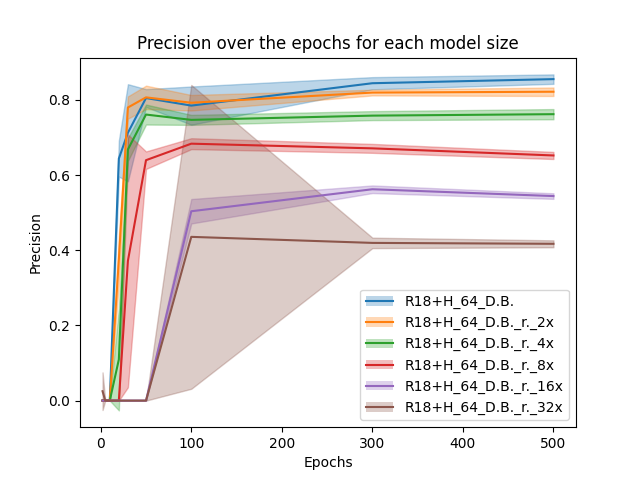
\includegraphics[width=1\linewidth]{Figures/results/resnet18+head/r18+h_precision_over_epochs_reduced_models.png}
      \captionof{figure}{Visualisation de la précision de ResNet18+Tête avec 64 blocs de détection (D.B.) pour les versions réduites.}
      \label{fig:resnet18+head_precision_reduced}
    \end{minipage}%
    \begin{minipage}[t]{.5\textwidth}%\vspace{5pt}
      \centering
      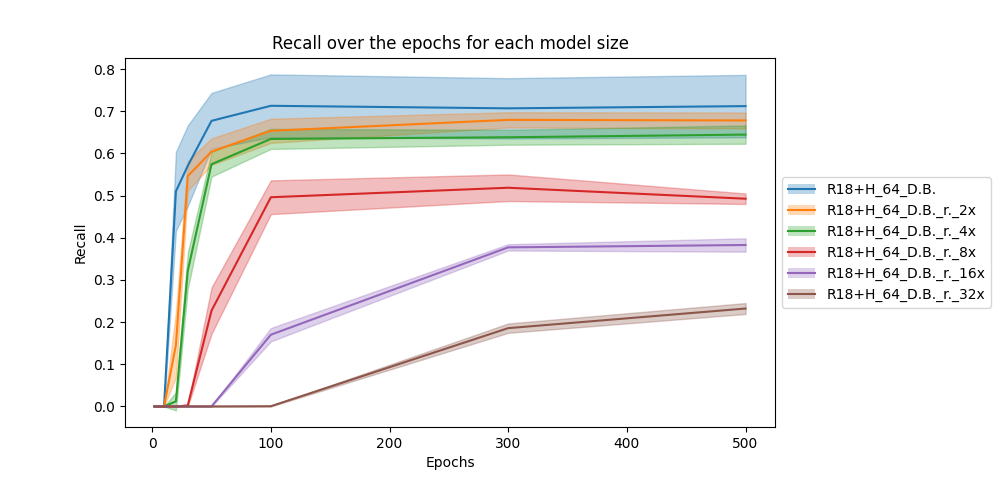
\includegraphics[width=1\linewidth ]{Figures/results/resnet18+head/r18+h_recall_over_epochs_reduced_models.png}
      \captionof{figure}{Visualisation du rappel de ResNet18+Tête avec 64 blocs de détection (D.B.) pour les versions réduites.}
      \label{fig:resnet18+head_recall_reduced}
    \end{minipage}
\end{figure}

\begin{figure}[!htbp]
    \centering
    \begin{minipage}[t]{.5\textwidth}%\vspace{0pt}
      \centering
      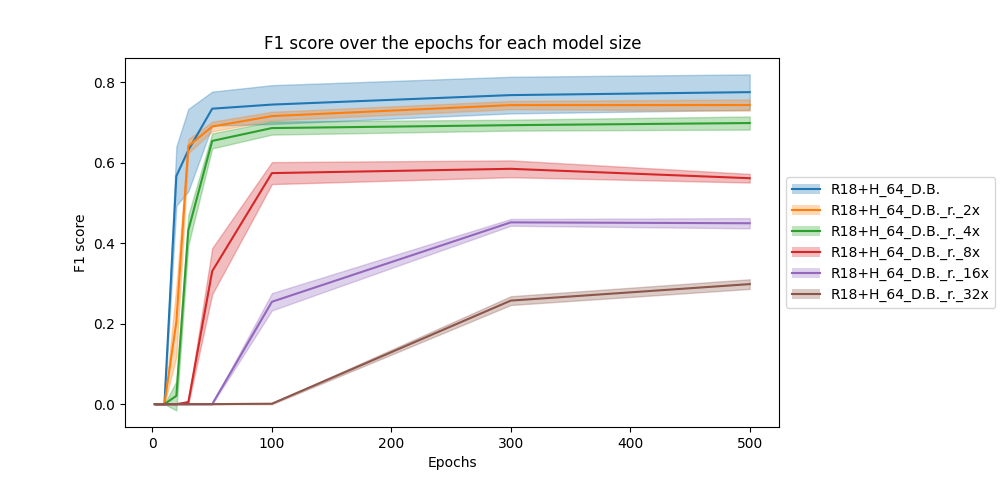
\includegraphics[width=1\linewidth]{Figures/results/resnet18+head/r18+h_f1_score_over_epochs_reduced_models.png}
      \captionof{figure}{Visualisation du score F1 de ResNet18+Tête avec 64 blocs de détection (D.B.) pour les versions réduites.}
      \label{fig:resnet18+head_f1_score_reduced}
    \end{minipage}%
\end{figure}

\begin{figure}[!htbp]
    \centering
    \begin{minipage}[t]{.5\textwidth}%\vspace{0pt}
      \centering
      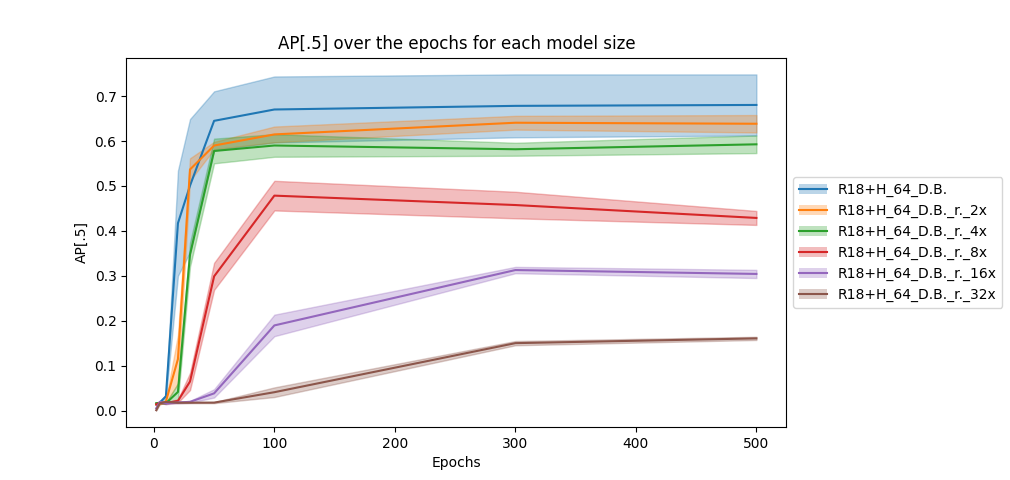
\includegraphics[width=1\linewidth]{Figures/results/resnet18+head/r18+h_ap05_over_epochs_reduced_models.png}
      \captionof{figure}{Visualisation de l'AP[.5] de ResNet18+Tête avec 64 blocs de détection (D.B.) pour les versions réduites.}
      \label{fig:resnet18+head_ap05_reduced}
    \end{minipage}%
    \begin{minipage}[t]{.5\textwidth}%\vspace{5pt}
      \centering
      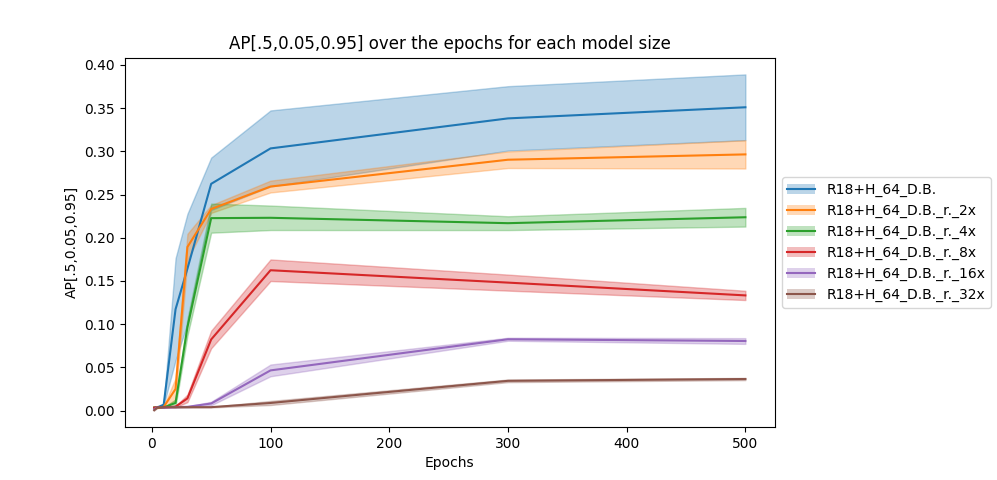
\includegraphics[width=1\linewidth ]{Figures/results/resnet18+head/r18+h_ap05_095_over_epochs_reduced_models.png}
      \captionof{figure}{Visualisation de l'AP[.5,.05,.95] de ResNet18+Tête avec 64 blocs de détection (D.B.) pour les versions réduites.}
      \label{fig:resnet18+head_ap05_095_reduced}
    \end{minipage}
\end{figure}

\break

Au niveau des performances, la table \ref{tab:max_values_for_each_metric_resnet18+head_reduced_models} nous montre les valeurs moyennes maximales toutes époques confondues pour les différentes métriques. Sur celle-ci, nous voyons que la diminution du nombre de filtres des couches de convolutions à un impact très important sur les résultats obtenus. En observant la différence entre le modèle de base et celui divisé par deux, nous observons entre 2 et 6\% d'écart, qui s'étend entre 9 et 13\% pour une division par quatre. Ce dernier, avec un score F1 de 69.82\% et une AP[.5] de 59.28\% qui sont des valeurs potentiellement acceptables, n'obtient que 22.37\% en moyenne pour l'AP[.5,.05,.95] qui est un score très pauvre.

Les versions encore plus petites obtiennent des valeurs encore plus faibles, démontrant les limites du modèle lorsque nous le réduisons.

\begin{table}[!ht]
    \caption{Valeurs moyennes maximales des métriques du modèle ResNet18+Tête avec 64 blocs de détection (D.B.) réduit toutes époques confondues}
    \label{tab:max_values_for_each_metric_resnet18+head_reduced_models}
    \rowcolors{2}{gray!25}{white}
    \centering
    \begin{tabular}{ |c||c|c|c|c|c|  }
        \hline
        \rowcolor{gray!50}
        Modèle & Précision & Rappel & Score F1 & AP[.5] & AP[.5,.05,.95]\\
        \hline
        R18+Tête 64 D.B & 0.8551 & 0.7129 & 0.7750 & 0.6804 & 0.3510\\
        R18+Tête 64 D.B. r. 2x & 0.8216 & 0.6795 & 0.7429 & 0.6409 & 0.2964\\
        R18+Tête 64 D.B. r. 4x & 0.7619 & 0.6446 & 0.6982 & 0.5928 & 0.2237\\
        R18+Tête 64 D.B. r. 8x & 0.6834 & 0.5186 & 0.5845 & 0.4785 & 0.1624\\
        R18+Tête 64 D.B. r. 16x & 0.5622 & 0.3828 & 0.4515 & 0.3129 & 0.0825\\
        R18+Tête 64 D.B. r. 32x & 0.4356 & 0.2322 & 0.2981 & 0.1607  & 0.0365\\
        \hline
    \end{tabular}
\end{table}

Au niveau de la courbe précision et rappel, celle-ci nous laisse voir sur la figure \ref{fig:resnet18+head_apxr_05_500_reduced} pour une \acrshort{iou} de 50\% que la version de base ainsi que celles réduites par deux, et quatre sont relativement proches. Puis les modèles encore plus réduits possèdent, à leur niveau, une relation plus pauvre. En regardant la même courbe pour une \acrshort{iou} de 95\% sur la figure \ref{fig:resnet18+head_apxr_095_500_reduced}, nous voyons que celle-ci est quasi nulle.

\begin{figure}[!htbp]
    \centering
    \begin{minipage}[t]{.5\textwidth}%\vspace{0pt}
      \centering
      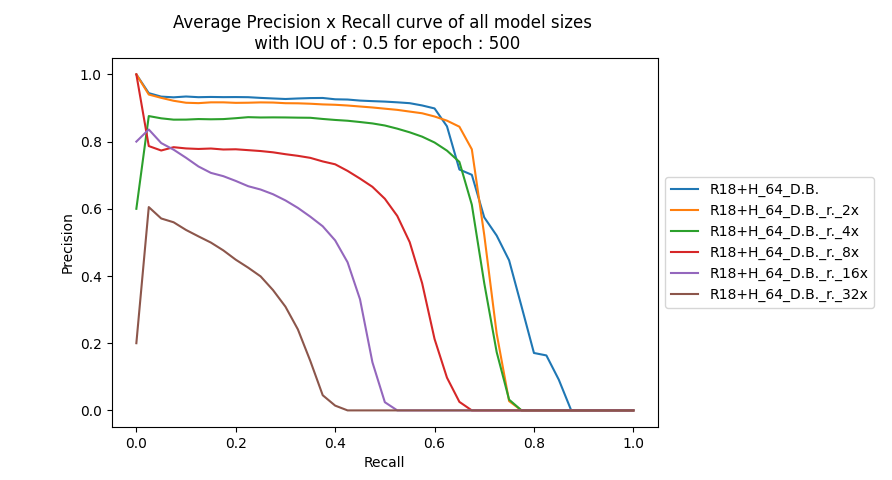
\includegraphics[width=1\linewidth]{Figures/results/resnet18+head/r18+h_apxr_05_500_reduced_models.png}
      \captionof{figure}{Visualisation de la moyenne des courbes précision x rappel avec un IoU de 0.5 pour les versions réduites de ResNet18+Tête avec 64 blocs de détection (D.B.) après 500 époques.}
      \label{fig:resnet18+head_apxr_05_500_reduced}
    \end{minipage}%
    \begin{minipage}[t]{.5\textwidth}%\vspace{5pt}
      \centering
      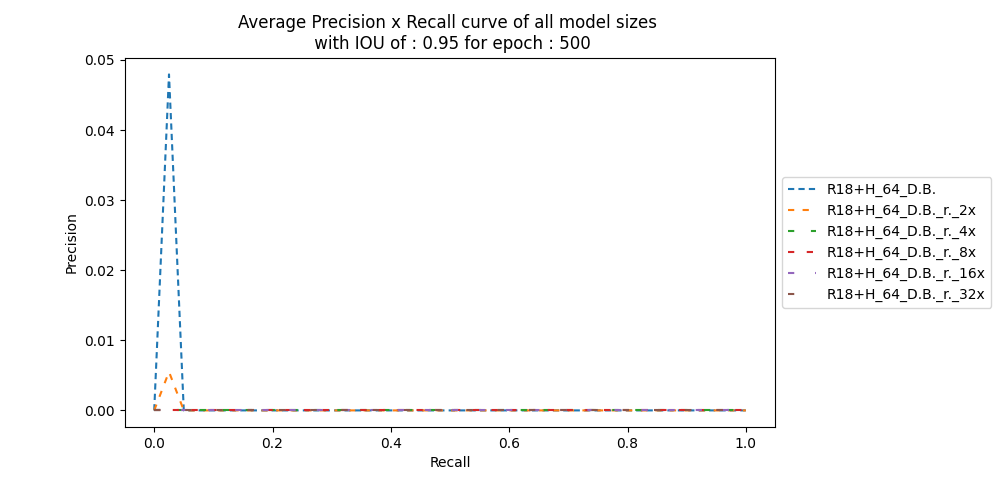
\includegraphics[width=1\linewidth ]{Figures/results/resnet18+head/r18+h_apxr_095_500_reduced_models.png}
      \captionof{figure}{Visualisation de la moyenne des courbes précision x rappel avec un IoU de 0.95 pour les versions réduites de ResNet18+Tête avec 64 blocs de détection (D.B.) après 500 époques.}
      \label{fig:resnet18+head_apxr_095_500_reduced}
    \end{minipage}
\end{figure}

\break

Bien que le modèle de base performe relativement bien, la réduction des filtres des couches de convolution est mal supportée par le modèle. Cependant en gardant en tête qu'il s'agit de base d'un modèle de classification que nous avons détourné pour en faire un modèle de détection en utilisant une tête très simple, celui-ci fonctionne plutôt bien.\\

Finalement, sur la table \ref{tab:resnet18+head_params_flops_vitesse_fps_reduced} nous retrouvons à nouveau une relation quadratique entre les différentes versions de ResNet18+Tête. Cela est vrai jusqu'à un certain facteur à partir duquel les paramètres d'autres couches deviennent significatifs.

En ce qui concerne la vitesse, nous observons un gain lors des premières réductions des filtres qui se stabilise par la suite. Le nombre de blocs de détection reste constant et comme nous l'avons vu précédemment, celui-ci influence la vitesse d'inférence du modèle. Nous supposons alors que malgré une forte diminution du nombre de paramètres et d'opérations, le modèle atteint ses limites, du moins sur la carte graphique utilisée, à cause du nombre de blocs de détection. À titre de comparaison, en travaillant avec ResNet18+Tête avec 16 blocs de détections et dont le nombre de filtres a été divisé par 16, nous obtenons un temps d'inférence de 0.093 ms ce qui donne 10748 images par secondes. La différence entre cette version réduite et celle non réduite est de plus de 2000 images par seconde contrairement à la version avec 64 blocs de détections dont l'écart est de moins de 600 images par secondes.

Néanmoins, dépassant rapidement les 5000 images par seconde avec un temps d'inférence inférieur à 0.2 ms, nous constatons que les variantes de notre modèle, avec des performances mitigées, sont capables de vitesses très intéressantes dans le cadre d'applications en temps réel.

\begin{table}[!ht]
    \caption{Nombre de paramètres, FLOPs, vitesse, FPS pour ResNet18+Tête avec 16, 64, et 121 blocs de détection (D.B)}
    \label{tab:resnet18+head_params_flops_vitesse_fps_reduced}
    \rowcolors{2}{gray!25}{white}
    \centering
    \begin{tabular}{ |c||c|c|c|c| }
        \hline
        \rowcolor{gray!50}
        Modèle & Paramètres (M) & MFLOPs & Vitesse (ms) RTX 4070 & FPS\\
        \hline
        R18+Tête 64 D.B. & 11.289408 & 287.530112 & 0.2142 & 4668\\
        R18+Tête 64 D.B. r. 2x & 2.855424 & 76.844704 & 0.2016 & 4960\\
        R18+Tête 64 D.B. r. 4x & 0.730464 & 21.692336 & 0.1974 & 5066\\
        R18+Tête 64 D.B. r. 8x & 0.190992 & 6.663736 & 0.1933 & 5171\\
        R18+Tête 64 D.B. r. 16x & 0.052008 & 2.286332 & 0.1920 & 5208\\
        R18+Tête 64 D.B. r. 32x & 0.015204 & 0.881854 & 0.1937 & 5161\\
        \hline
    \end{tabular}
\end{table}

\break

\subsection{Résultats ResNet18+Tête : version quantifiée avec 64 blocs de détection}

Étant donné que nous souhaitons synthétiser notre modèle ResNet18+Tête à l'aide de HLS4ML en vue d'une implémentation sur \acrshort{fpga}, nous avons d'abord quantifié ce dernier à l'aide de QKeras afin d'obtenir le réseau de neurones le plus proche du résultat final.

Notre version fraîchement quantifiée de ResNet18+Tête avec 64 blocs de détection est malheureusement plus lente en termes de vitesse de calculs. Cela est notamment dû au fait qu'elle n'arrive pas à profiter des unités de calculs de la carte graphique destinées aux virgules flottantes, car elle utilise une représentation en virgule fixe. Afin de gagner du temps, il est possible de réaliser de l'apprentissage par transfert en utilisant les poids du modèle à virgule flottante comme base afin d'accélérer l'entraînement, plutôt que d'en réaliser un nouveau à partir de poids initialisé aléatoirement.\\

Les figures \ref{fig:qresnet18+head_precision}, \ref{fig:qresnet18+head_recall}, \ref{fig:qresnet18+head_f1_score}, \ref{fig:qresnet18+head_ap05}, \ref{fig:qresnet18+head_ap05_095}, \ref{fig:qresnet18+head_apxr_05_500}, et \ref{fig:qresnet18+head_apxr_095_500} nous permettent de voir l'évolution du modèle pour nos différentes métriques au fil des $500$ premières époques de l'entraînement de la version de base, ainsi que de ses alternatives quantifiées sur 8 et 16 bits réutilisant des poids, ou à partir de zéro. Ces dernières ont été entraînées sur mille époques, mais pour des soucis de visibilité sur les figures elles ne seront pas représentées. Néanmoins, leurs résultats sont accessibles aux tables \ref{appendix:qresnet18_8b_fs}, et \ref{appendix:qresnet18_8b_fs} en annexes.

\begin{figure}[!htbp]
    \centering
    \begin{minipage}[t]{.5\textwidth}%\vspace{0pt}
      \centering
      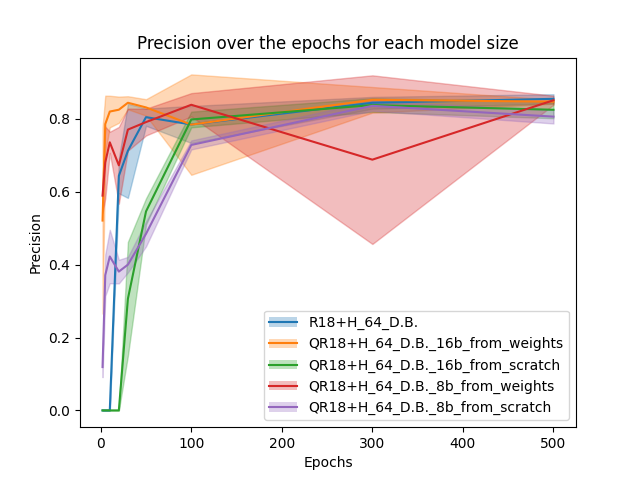
\includegraphics[width=1.1\linewidth]{Figures/results/qresnet18+head/qr18+h_precision_over_epochs_500.png}
      \captionof{figure}{Visualisation de la précision de ResNet18+Tête avec 64 blocs de détection (D.B.) et ses versions quantifiées de 8 et 16 bits.}
      \label{fig:qresnet18+head_precision}
    \end{minipage}%
    \begin{minipage}[t]{.5\textwidth}%\vspace{5pt}
      \centering
      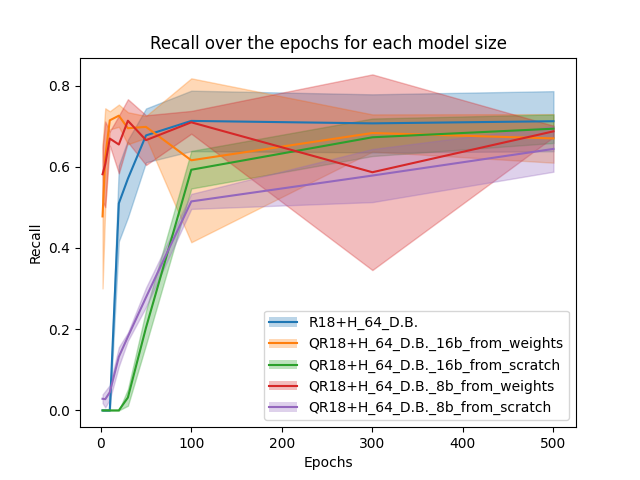
\includegraphics[width=1.1\linewidth ]{Figures/results/qresnet18+head/qr18+h_rappel_over_epochs_500.png}
      \captionof{figure}{Visualisation du rappel de ResNet18+Tête avec 64 blocs de détection (D.B.) et ses versions quantifiées de 8 et 16 bits.}
      \label{fig:qresnet18+head_recall}
    \end{minipage}
\end{figure}

\begin{figure}[!htbp]
    \centering
    \begin{minipage}[t]{.5\textwidth}%\vspace{0pt}
      \centering
      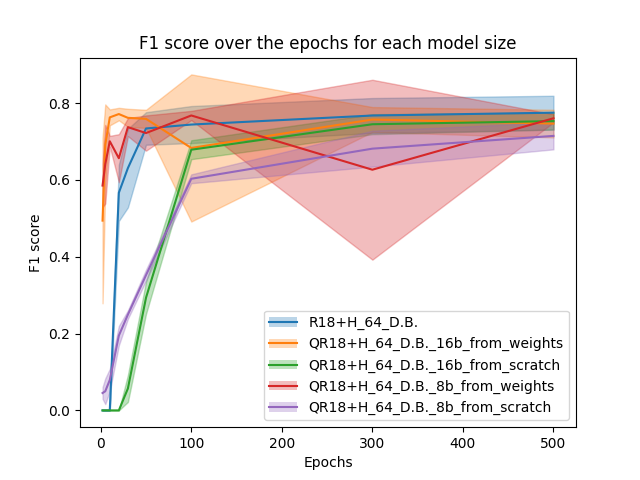
\includegraphics[width=1.1\linewidth]{Figures/results/qresnet18+head/qr18+h_f1_score_over_epochs_500.png}
      \captionof{figure}{Visualisation du score F1 de ResNet18+Tête avec 64 blocs de détection (D.B.) et ses versions quantifiées de 8 et 16 bits.}
      \label{fig:qresnet18+head_f1_score}
    \end{minipage}%
\end{figure}

\begin{figure}[!htbp]
    \centering
    \begin{minipage}[t]{.5\textwidth}%\vspace{0pt}
      \centering
      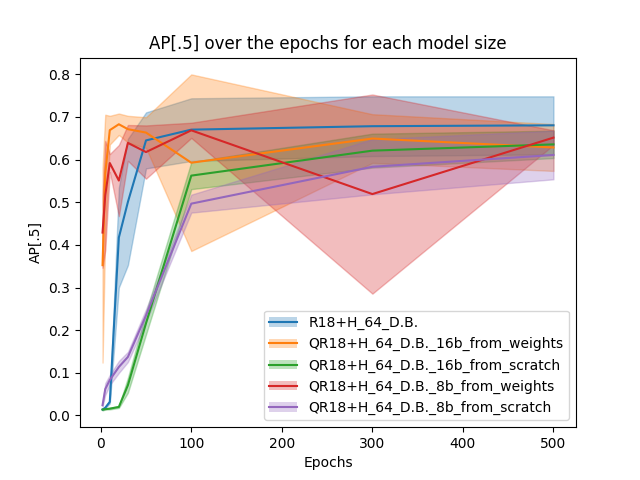
\includegraphics[width=1.1\linewidth]{Figures/results/qresnet18+head/qr18+h_ap05_over_epochs_500.png}
      \captionof{figure}{Visualisation de l'AP[.5] de ResNet18+Tête avec 64 blocs de détection (D.B.) et ses versions quantifiées de 8 et 16 bits.}
      \label{fig:qresnet18+head_ap05}
    \end{minipage}%
    \begin{minipage}[t]{.5\textwidth}%\vspace{5pt}
      \centering
      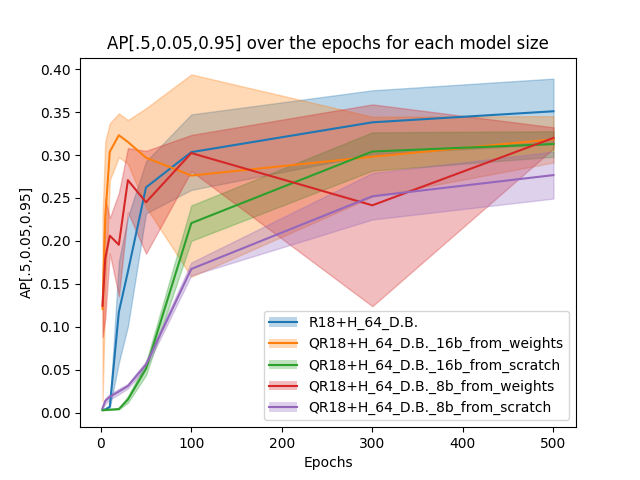
\includegraphics[width=1.1\linewidth ]{Figures/results/qresnet18+head/qr18+h_ap05_095_over_epochs_500.png}
      \captionof{figure}{Visualisation de l'AP[.5,.05,.95] de ResNet18+Tête avec 64 blocs de détection (D.B.) et ses versions quantifiées de 8 et 16 bits.}
      \label{fig:qresnet18+head_ap05_095}
    \end{minipage}
\end{figure}

\break

Lorsque nous observons les différentes figures, nous constatons effectivement qu'à partir des poids initialisés aléatoirement les versions quantifiées sur 8 et 16 bits nécessitent plus d'époques d'entraînement pour atteindre des performances similaires. En réutilisant les poids des versions à virgules flottantes, nous voyons qu'il faut effectivement peu d'époques pour atteindre en moyenne des résultats similaires. Cependant, un point intéressant à relever est l'écart type qui est plus élevé sur les modèles réutilisant des poids que sur ceux apprenant à partir de zéro.

Cela est très certainement dû aux poids optimisés pour une représentation à virgule flottante. La perte de précision générée par la quantification demande au modèle d'affiner ses poids dans une résolution à virgule fixe. Celui-ci doit s'adapter à une nouvelle représentation introduisant alors une certaine instabilité. À l'inverse, lors d'un entraînement depuis le début, le modèle va s'adapter plus progressivement et, comme nous pouvons le voir sur les figures, sera plus stable.\\

Bien qu'il y ait quelques pour cent d'écart, les figures nous montrent que les différentes versions évoluent vers des résultats plutôt proches. Au niveau des différentes métriques, nous voyons qu'elles ont toutes des résultats relativement proches. Cependant, bien que cela ne soit pas visible sur la figure affichant la précision, le modèle le plus performant reste la version à virgule flottante, et le moins bon semble être la version quantifiée sur 8 bits entraînés à partir de zéro. Les autres versions sont plus complexes à analyser sur les figures, nous étudierons leur comportement plus loin avec les valeurs moyennes maximales.\\

En ce qui concerne la relation de la précision avec le rappel pour une \acrshort{iou} de 50\%, nous voyons sur la figure \ref{fig:qresnet18+head_apxr_05_500}, que le comportement est relativement similaire à celui du modèle de base, avec une légère baisse de la qualité de la précision en fonction du rappel. Il reste néanmoins très bon.

Avec une \acrshort{iou} de 95\% sur la figure \ref{fig:qresnet18+head_apxr_095_500}, nous voyons que celle-ci est toujours aussi mauvaise pour la version quantifiée sur 16 bits, mais surprenamment, bien que le modèle quantifié sur 8 bits soit également mauvais, il semble performer mieux lors d'un très faible rappel. Il est possible qu'avec une représentation sur 8 bits le modèle arrive à mieux généraliser ce qui lui confère de légères meilleures performances lors d'une intersection sur union plus élevée. Néanmoins, malgré les pauvres résultats obtenus sur cette courbe, nous voyons que les versions quantifiées s'en tirent au moins aussi bien que celle de base.\\

\begin{figure}[!htbp]
    \centering
    \begin{minipage}[t]{.5\textwidth}%\vspace{0pt}
      \centering
      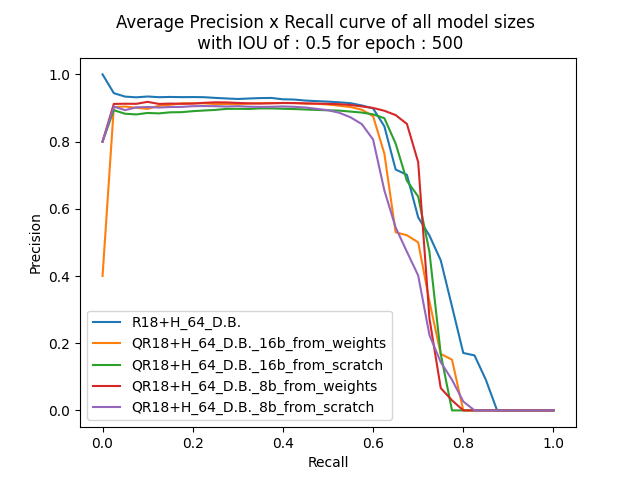
\includegraphics[width=1.1\linewidth]{Figures/results/qresnet18+head/qr18+h_apxr_05_500.png}
      \captionof{figure}{Visualisation de la moyenne des courbes précision x rappel avec un IoU de 0.5 pour les versions quantifiées de 8 et 16 bits de ResNet18+Tête avec 64 blocs de détection (D.B.) après 500 époques.}
      \label{fig:qresnet18+head_apxr_05_500}
    \end{minipage}%
    \begin{minipage}[t]{.5\textwidth}%\vspace{5pt}
      \centering
      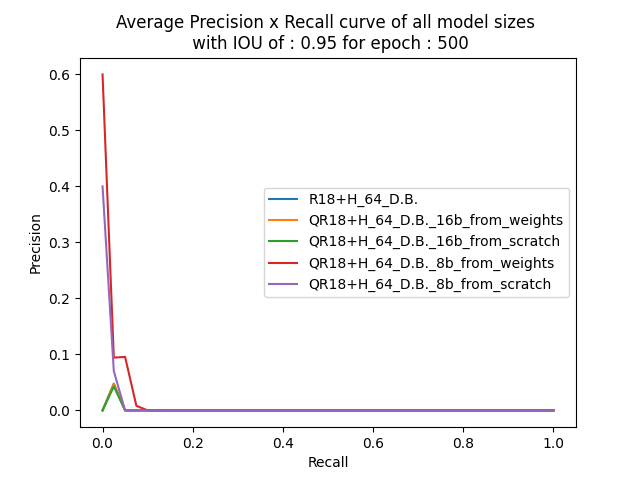
\includegraphics[width=1.1\linewidth ]{Figures/results/qresnet18+head/qr18+h_apxr_05_095_500.png}
      \captionof{figure}{Visualisation de la moyenne des courbes précision x rappel avec un IoU de 0.95 pour les versions quantifiées de 8 et 16 bits de ResNet18+Tête avec 64 blocs de détection (D.B.) après 500 époques.}
      \label{fig:qresnet18+head_apxr_095_500}
    \end{minipage}
\end{figure}

Analysons à présent les valeurs moyennes maximums de chaque version pour chaque métrique toutes époques confondues disponibles sur la table \ref{tab:max_values_for_each_metric_qresnet18+head_models}. Nous voyons que les versions quantifiées obtiennent des performances relativement proches du modèle à représentation en virgule flottante. Entre les différentes versions, il n'y a que quelques pourcentages de différence à travers toutes les métriques. Cependant, le modèle sur 8 bits performe légèrement moins bien que celui sur 16 bits dans toutes les métriques excepté la précision. Ce dernier possède des valeurs relativement proches, voire équivalentes au modèle de base, bien que sur l'AP[.5,.05,.95], nous observons une plus grosse différence.

De plus, la différence entre les versions quantifiées pré-entrainées et celles entraînées de zéro est très faible alors que ces dernières affichent des valeurs tirées parmi les résultats au bout de plus de $500$ époques, confirmant à nouveau que l'utilisation de poids à virgule flottante pré-entraînés accélère l'entraînement des versions quantifiées.

Ainsi, avec un score F1 de 77.14\%, une AP[.5] de 68\%, et une AP[.5,.05,.95] de 32\%, la version quantifiée de ResNet18+Tête sur 16 bits présente des performances quasi identiques au modèle de base, qui sont relativement bonnes. C'est cette version que nous allons ajuster et utiliser avec le paquet HLS4ML.

\begin{table}[!ht]
    \caption{Valeurs moyennes maximales des métriques du modèle ResNet18+Tête avec 64 blocs de détection (D.B.) quantifié sur 8 ou 16 bits à partir de poids préentrainés sur un modèle à virgule flottante et à partir de zéro}
    \label{tab:max_values_for_each_metric_qresnet18+head_models}
    \rowcolors{2}{gray!25}{white}
    \centering
    \begin{tabular}{ |c||c|c|c|c|c|  }
        \hline
        \rowcolor{gray!50}
        Modèle & Précision & Rappel & Score F1 & AP[.5] & AP[.5,.05,.95]\\
        \hline
        R18+Tête 64 D.B & 0.8551 & 0.7129 & 0.7750 & 0.6804 & 0.3510\\
        \begin{tabular}{@{}c@{}}QR18+Tête 64 D.B. \\ 8 bits pré-entrainé\end{tabular} & 0.8512 & 0.7134 & 0.7677 & 0.6687 & 0.3200\\
        \begin{tabular}{@{}c@{}}QR18+Tête 64 D.B. \\ 8 bits de zéro\end{tabular} & 0.8360 & 0.6963 & 0.7582 & 0.6683 & 0.3031\\
        \begin{tabular}{@{}c@{}}QR18+Tête 64 D.B. \\ 16 bits pré-entrainé\end{tabular} & 0.8473 & 0.7258 & 0.7714 & 0.6830 & 0.3231\\
        \begin{tabular}{@{}c@{}}QR18+Tête 64 D.B. \\ 16 bits de zéro\end{tabular} & 0.8551 & 0.7131 & 0.7769 & 0.6616 & 0.3387\\
        \hline
    \end{tabular}
\end{table}

\subsection{Résultats ResNet18+Tête : version quantifiée pour HLS4ML}

Comme nous avons pu le voir précédemment, la version de notre modèle quantifié sur 16 bits semble être adaptée pour notre cas. Afin de pouvoir l'utiliser avec HLS4ML, nous avons dû réduire la taille de celui-ci afin de permettre à l'outil d'optimiser la latence. Pour cela, nous avons décidé d'utiliser la version réduisant le nombre de filtres par convolution par seize. Malgré ses maigres performances, celui-ci nous permet de maximiser le nombre de couches utilisant la stratégie "latence", tout en limitant les ressources matérielles nécessaires pour aboutir à la synthèse.

Cependant, HLS4ML ne supporte malheureusement pas l'utilisation de stride dans la couche de MaxPooling. Afin de pouvoir tout de même synthétiser notre modèle, nous avons retiré ce stride.\\

Cette sous-section a donc pour but de présenter les performances de la version quantifiée puis synthétisée avec HLS4ML. Les figures \ref{fig:qresnet18+head_precision_wo_stride}, \ref{fig:qresnet18+head_recall_wo_stride}, \ref{fig:qresnet18+head_f1_score_wo_stride}, \ref{fig:qresnet18+head_ap05_wo_stride}, \ref{fig:qresnet18+head_ap05_095_wo_stride}, \ref{fig:qresnet18+head_apxr_05_500_wo_stride}, et \ref{fig:qresnet18+head_apxr_095_500_wo_stride} affichent les résultats de la version de base dont les filtres de convolution ont été réduits seize fois, ainsi que sa version quantifiée aux côtés des mêmes modèles dont le stride à la couche MaxPooling a été retirée. L'entraînement des versions quantifiées a été réalisé à partir des poids des versions à virgule flottante.

\begin{figure}[!htbp]
    \centering
    \begin{minipage}[t]{.5\textwidth}%\vspace{0pt}
      \centering
      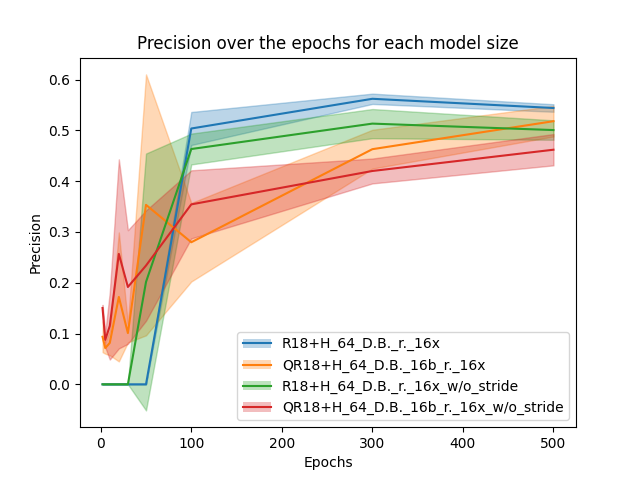
\includegraphics[width=1.1\linewidth]{Figures/results/qresnet18+head/qr18+h_precision_over_epochs_500_wo_stride.png}
      \captionof{figure}{Visualisation de la précision de ResNet18+Tête avec 64 blocs de détection (D.B.) pour sa version quantifiée sur 16 bits réduite 16 fois avec et sans MaxPooling stride.}
      \label{fig:qresnet18+head_precision_wo_stride}
    \end{minipage}%
    \begin{minipage}[t]{.5\textwidth}%\vspace{5pt}
      \centering
      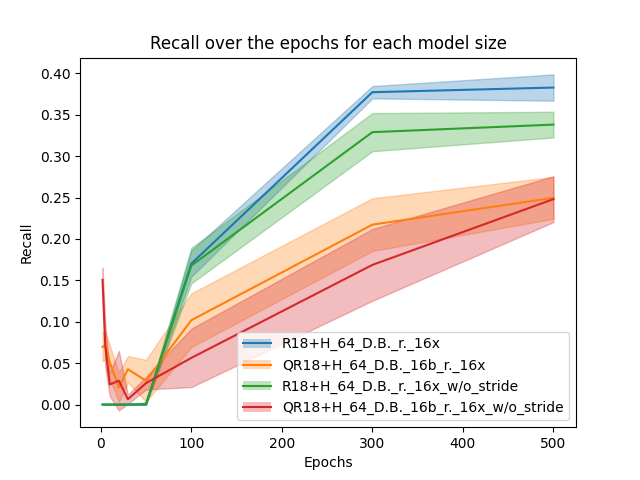
\includegraphics[width=1.1\linewidth ]{Figures/results/qresnet18+head/qr18+h_rappel_over_epochs_500_wo_stride.png}
      \captionof{figure}{Visualisation du rappel de ResNet18+Tête avec 64 blocs de détection (D.B.) pour sa version quantifiée sur 16 bits réduite 16 fois avec et sans MaxPooling stride.}
      \label{fig:qresnet18+head_recall_wo_stride}
    \end{minipage}
\end{figure}

\begin{figure}[!htbp]
    \centering
    \begin{minipage}[t]{.5\textwidth}%\vspace{0pt}
      \centering
      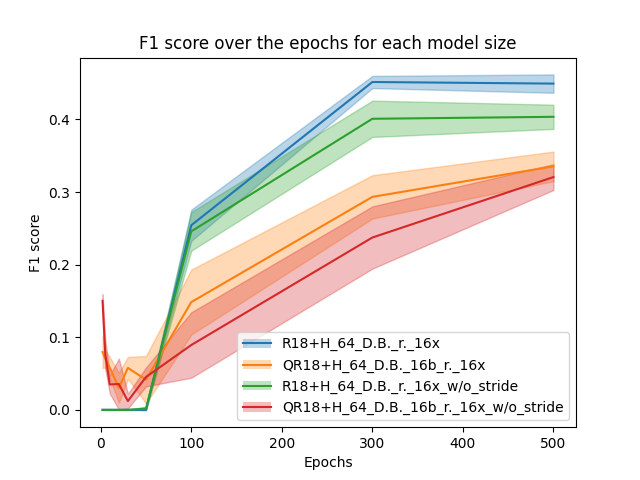
\includegraphics[width=1.1\linewidth]{Figures/results/qresnet18+head/qr18+h_f1_score_over_epochs_500_wo_stride.png}
      \captionof{figure}{Visualisation du score F1 de ResNet18+Tête avec 64 blocs de détection (D.B.) pour sa version quantifiée sur 16 bits réduite 16 fois avec et sans MaxPooling stride.}
      \label{fig:qresnet18+head_f1_score_wo_stride}
    \end{minipage}%
\end{figure}

\begin{figure}[!htbp]
    \centering
    \begin{minipage}[t]{.5\textwidth}%\vspace{0pt}
      \centering
      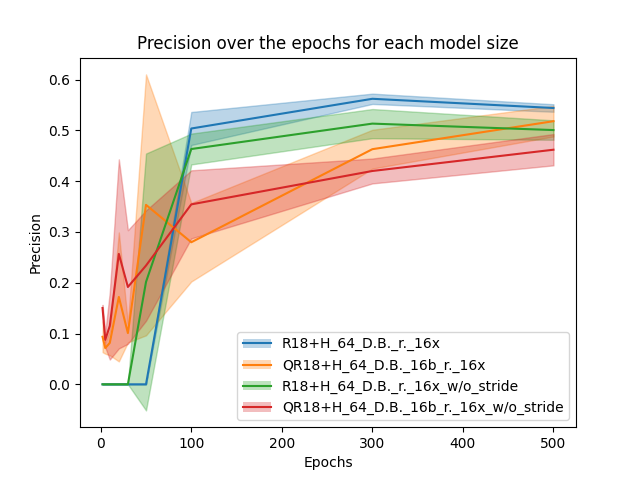
\includegraphics[width=1.1\linewidth]{Figures/results/qresnet18+head/qr18+h_precision_over_epochs_500_wo_stride.png}
      \captionof{figure}{Visualisation de l'AP[.5] de ResNet18+Tête avec 64 blocs de détection (D.B.) pour sa version quantifiée sur 16 bits réduite 16 fois avec et sans MaxPooling stride.}
      \label{fig:qresnet18+head_ap05_wo_stride}
    \end{minipage}%
    \begin{minipage}[t]{.5\textwidth}%\vspace{5pt}
      \centering
      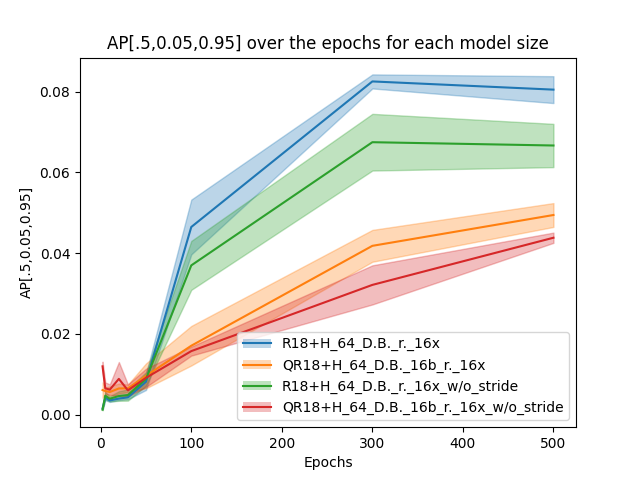
\includegraphics[width=1.1\linewidth ]{Figures/results/qresnet18+head/qr18+h_ap05_095_over_epochs_500_wo_stride.png}
      \captionof{figure}{Visualisation de l'AP[.5,.05,.95] de ResNet18+Tête avec 64 blocs de détection (D.B.) pour sa version quantifiée sur 16 bits réduite 16 fois avec et sans MaxPooling stride.}
      \label{fig:qresnet18+head_ap05_095_wo_stride}
    \end{minipage}
\end{figure}

\break

Nous remarquons immédiatement la perte de performances entre les versions à représentation flottante et fixe. De plus, nous constatons également une diminution des résultats pour les versions n'utilisant pas de stride. Cependant, il est intéressant de noter que cette différence est plus prononcée pour les versions à virgule flottante que celles à virgule fixe. Finalement, tout comme pour les variantes de ResNet18+Tête réalisées, nous voyons sur les courbes de précisions et de rappel que lors d'une intersection sur union de 50\% sur la figure \ref{fig:qresnet18+head_apxr_05_500_wo_stride}, même si celle-ci est pauvre, elle demeure capable d'obtenir une certaine précision tant que le rappel n'est pas trop élevé. En revanche, dès que l'\acrshort{iou} passe à 95\%, la courbe est inexistante, comme visible sur la figure \ref{fig:qresnet18+head_apxr_095_500_wo_stride}.

\begin{figure}[!htbp]
    \centering
    \begin{minipage}[t]{.5\textwidth}%\vspace{0pt}
      \centering
      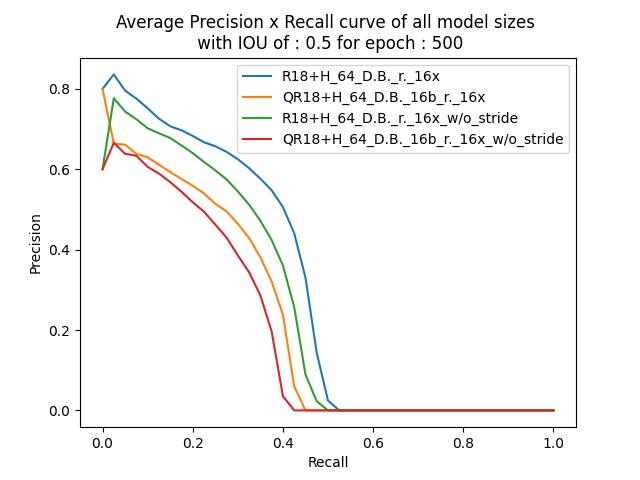
\includegraphics[width=1.1\linewidth]{Figures/results/qresnet18+head/qr18+h_apxr_05_500_wo_stride.png}
      \captionof{figure}{Visualisation de la moyenne des courbes précision x rappel avec un IoU de 0.5 pour la version quantifiée sur 16 bits avec et sans MaxPooling stride de ResNet18+Tête avec 64 blocs de détection (D.B.) réduite 16 fois après 500 époques.}
      \label{fig:qresnet18+head_apxr_05_500_wo_stride}
    \end{minipage}%
    \begin{minipage}[t]{.5\textwidth}%\vspace{5pt}
      \centering
      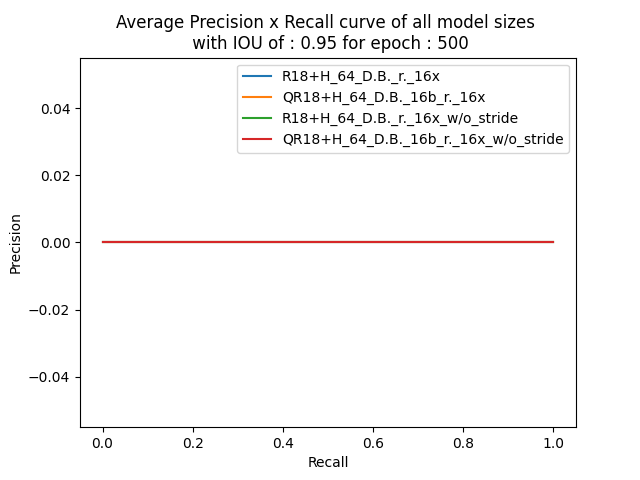
\includegraphics[width=1.1\linewidth ]{Figures/results/qresnet18+head/qr18+h_apxr_05_095_500_wo_stride.png}
      \captionof{figure}{Visualisation de la moyenne des courbes précision x rappel avec un IoU de 0.95 pour la version quantifiée sur 16 bits avec et sans MaxPooling stride de ResNet18+Tête avec 64 blocs de détection (D.B.) réduite 16 fois après 500 époques.}
      \label{fig:qresnet18+head_apxr_095_500_wo_stride}
    \end{minipage}
\end{figure}

\break

Retirer le stride à la couche de MaxPooling à plusieurs impacts. Celui-ci sert notamment à réduire la dimensionnalité de l'entrée de la couche permettant de mieux capturer les caractéristiques et de réduire les informations non pertinentes, telles que le bruit. Mais, il permet également de réduire le nombre de calculs à réaliser par la suite.

Même si la différence entre les versions quantifiées n'est pas très importante, il est dommage de perdre ces pourcentages lors de l'étape de synthèse. Cependant, afin de pouvoir aboutir à un résultat, nous allons utiliser cette version sans stride.

\section{Comparaison des résultats entre YOLOv8 et Resnet18 + Tête}

Comparons à présent les deux modèles utilisés dans ce travail. Sans surprises, YOLOv8, le modèle développé pour effectuer de la détection d'objets performe sans aucun doute mieux que la version ResNet18+Tête en termes de précision, rappel, score F1, et précision moyenne. Avec des résultats élevés et une faculté à réaliser des détections même avec de grandes contraintes d'intersection sur union, il ne fait aucun doute que YOLOv8 est un modèle très puissant et plus que capable de réaliser la détection de jets. De plus, comme nous avons pu le voir, même les versions réduites de celui-ci sont capables d'obtenir des résultats corrects avec une perte de performances acceptable.

De l'autre côté, bien que moins performant, ResNet18+Tête démontre qu'un modèle de classification modifié pour réaliser de la détection est également capable d'obtenir des résultats satisfaisants. Cependant, contrairement à YOLOv8, ce dernier supporte moins bien la réduction du nombre de filtres de ses couches de convolution, dégradant assez fortement ses performances. Néanmoins, ResNet18+Tête se démarque face à YOLOv8, notamment au niveau de la vitesse qu'il est capable d'atteindre, mais aussi de par son implémentation plus simple qui permet de facilement le modifier, notamment afin de l'adapter à son utilisation avec HLS4ML.

Ainsi, malgré les performances plus élevées avec le modèle YOLOv8, les limitations rencontrées avec \acrshort{hls4ml} font de ResNet18+Tête un choix intéressant dans des contraintes de performances en temps réel très exigeantes.

\section{Synthèse du modèle réduit QResnet18+Tête avec HLS4ML}

Afin de synthétiser notre modèle avec HLS4ML, nous avons dû installer l'outil Vitis HLS. Pour des raisons d'espace mémoire sur la machine utilisée, nous avons utilisé la version 2022.1. Celle-ci inclut par défaut plusieurs types de \acrshort{fpga}. Cependant, de par la taille de notre réseau de neurones, nous souhaitons synthétiser notre code pour le modèle U250 \cite{noauthor_alveo_nodate} de la famille Alveo. Ces cartes ont été développées afin de répondre aux besoins des centres de données, et proposent de meilleures performances que les processeurs notamment dans le domaine de l'inférence de modèles de machine learning. La carte utilisée possède 5376 \acrfull{bram}, 12288 \acrfull{dsp}, 3456000 \acrfull{ff}, et 1728000 \acrfull{lut}. De plus, les cycles d'horloges de notre projet ont été laissés à la valeur par défaut, c'est-à-dire $5 \: ns$.

Lorsque nous synthétisons notre modèle avec HLS4ML, le paquet va créer un dossier contenant tous les éléments qu'il a générés. Parmi ceux-ci, nous retrouvons le code VHDL, Verilog, ainsi qu'un dossier nommé "report" contenant des fichiers .rpt donnant les détails de chaque couche synthétisée, comme la latence, le nombre de ressources utilisées, etc.. Parmi ces fichiers, nous retrouvons un résumé de la totalité du modèle.\\

La version synthétisée, QResNet18+Tête sans MaxPooling stride divisée par 16, nous affiche les résultats présentés sur la table \ref{tab:resources_and_latency_by_reuse_factor}. Nous pouvons voir sur celle-ci des valeurs différentes en fonction du "reuse factor" utilisé pour 1, 10, 100, et 1000. Celui-ci permet d'indiquer à l'outil le nombre de fois qu'un bloc de calcul doit être réutilisé.

Ainsi, nous voyons que le nombre de \acrshort{dsp} diminue lorsque nous augmentons le nombre de réutilisations. Cependant, diminuer le nombre de \acrshort{dsp} augmente la latence de notre système. Cela est logique étant donné qu'attribuer un "reuse factor" de $1$, revient à paralléliser l'ensemble des opérations à effectuer, mais demande un nombre de ressources très conséquentes. Comme nous pouvons le voir sur la table, ne pas réutiliser de \acrshort{dsp} demande l'utilisation d'un nombre trop élevé de ces derniers. Synthétiser notre modèle demande donc de trouver le subtil équilibre entre la parallélisation des calculs et les ressources à disposition, en acceptant d'augmenter la latence.

Par ailleurs, nous constatons que lorsque nous diminuons le nombre de \acrshort{dsp}, nous augmentons le nombre de \acrshort{ff}, et de \acrshort{lut} utilisés. En effet, les \acrshort{ff} vont permettre de temporiser les calculs qui doivent être effectués par un nombre plus restreint de \acrshort{dsp}, tandis que les \acrshort{lut} vont pouvoir réaliser des fonctions relativement simples.\\

Une autre mesure est l'\acrfull{ii}, qui indique le nombre de cycles d'horloges (\acrfull{cc}) requis avant que l'algorithme accepte une nouvelle entrée. Comme nous pouvons le constater, celle-ci est relativement proche de la latence lorsque le "reuse factor" est plutôt faible. Cependant, lorsque celui-ci augmente et devient assez grand comme pour le cas à $1000$, nous remarquons que l'\acrshort{ii} peut indiquer un temps beaucoup plus court que la latence. Ceci peut s'expliquer de par le fait que les opérations sont pipelinées efficacement aux côtés d'une conception traitant les entrées par étapes plutôt que parallèlement.

Le "reuse factor" de $1000$ a donc une latence plus élevée, mais propose dans le meilleur des cas un débit plus élevé que les versions pour lesquelles le "reuse factor" est de $100$ ou de $10$.\\

Finalement, à l'aide de notre table \ref{tab:resources_and_latency_by_reuse_factor}, nous voyons qu'utiliser un "reuse factor" de 10 permet de synthétiser notre modèle sur l'U250 avec une latence de 0.167 ms et un \acrshort{ii} tout aussi proche. Il s'agit là d'un très bon compromis qui pourrait être encore un peu optimisé en diminuant progressivement le "reuse factor".

\begin{table}[!ht]
    \caption{Ressouces et latence du modèle synthétisé par HLS4ML pour la \acrshort{fpga} Alveo U250 en fonction du "reuse factor"}
    \label{tab:resources_and_latency_by_reuse_factor}
    \rowcolors{2}{gray!25}{white}
    \centering
    \begin{tabular}{ |c||c|c|c|c|c|c|  }
        \hline
        \rowcolor{gray!50}
        \begin{tabular}{@{}c@{}}Reuse \\ factor\end{tabular} & \begin{tabular}{@{}c@{}}BRAM \\ (\%)\end{tabular} &      \begin{tabular}{@{}c@{}}DSP \\ (\%)\end{tabular} & \begin{tabular}{@{}c@{}}FF \\ (\%)\end{tabular} &        \begin{tabular}{@{}c@{}}LUT \\ (\%)\end{tabular} & Latency (\acrshort{cc}) & \acrshort{ii}                  (\acrshort{cc})\\
        \hline
        1 & \begin{tabular}{@{}c@{}}60 \\ (1\%)\end{tabular} & 
            \begin{tabular}{@{}c@{}}19767 \\ (160\%)\end{tabular} & 
            \begin{tabular}{@{}c@{}}373645 \\ (10\%)\end{tabular} & 
            \begin{tabular}{@{}c@{}}1523896 \\ (88\%)\end{tabular} & 
            \begin{tabular}{@{}c@{}}4813 \\ (24.065 $\mu{s}$)\end{tabular} & 
            4775\\
        10 & \begin{tabular}{@{}c@{}}60 \\ (1\%)\end{tabular} & 
            \begin{tabular}{@{}c@{}}4438 \\ (36\%)\end{tabular} & 
            \begin{tabular}{@{}c@{}}456833 \\ (13\%)\end{tabular} & 
            \begin{tabular}{@{}c@{}}1651718 \\ (95\%)\end{tabular} & 
            \begin{tabular}{@{}c@{}}33395 \\ (0.167 ms)\end{tabular} & 
            33330\\
        100 & \begin{tabular}{@{}c@{}}60 \\ (1\%)\end{tabular} & 
            \begin{tabular}{@{}c@{}}456 \\ (3\%)\end{tabular} & 
            \begin{tabular}{@{}c@{}}618873 \\ (20\%)\end{tabular} & 
            \begin{tabular}{@{}c@{}}1584404 \\ (93\%)\end{tabular} &
            \begin{tabular}{@{}c@{}}257281 \\ (1.286 ms)\end{tabular} & 
            257097\\
        1000 & \begin{tabular}{@{}c@{}}60 \\ (1\%)\end{tabular} &
            \begin{tabular}{@{}c@{}}60 \\ ($\sim$ 0\%)\end{tabular} & 
            \begin{tabular}{@{}c@{}}705668 \\ (20\%)\end{tabular} & 
            \begin{tabular}{@{}c@{}}1611532 \\ (93\%)\end{tabular} &
            \begin{tabular}{@{}c@{}}min : \\ 1618790 \\ (8.094 ms) \\ max : \\ 1619169 \\ (8.096 ms)\end{tabular} &
            \begin{tabular}{@{}c@{}}min : \\ 14285 \\ max : \\ 1618742 \end{tabular}\\
        \hline
    \end{tabular}
\end{table}

%----------------------------------------------------------------------------------------
